\chapter{z\LaTeX{}系列}
\section{简介}
\subsection{为何叫z?}
也不知道为什么这个系列名称要加以`z'的前缀,可能是因为个人爱好,或是因为觉得这个字母对自己而言有着一些别的意味。
最开始此系列中此包含一个基本的文档类,叫做 $\pi$\LaTeX{}, 但是后面自己想开发一个用于绘图的宏包,主要基于TiKZ.
用于常见平面图形的绘制以及外部程序的交互. 也许是看到了\cmd{tikz}库名称中的``z'',于是便以`z'为前缀,产生了
z\LaTeX{}\index{z\LaTeX{}}系列。


\subsection{项目地址}
目前本项目已经在GitHub, Gitlab, Gitee上开源,地址如下:
\begin{itemize}
    \item GitHub: \href{https://github.com/zongpingding/ZLaTeX_ZTikZ}{https://github.com/zongpingding/ZLaTeX\_ZTikZ}
    \item Gitlab: \href{https://gitlab.com/zongpingding/ZLaTeX_ZTikZ}{https://gitlab.com/zongpingding/ZLaTeX\_ZTikZ}
    \item Gitee:  \href{https://gitee.com/zongpingding/ZLaTeX_ZTikZ}{https://gitee.com/zongpingding/ZLaTeX\_ZTikZ}
\end{itemize}

项目中包含z\LaTeX{}文档类源码\cmd{zlatex.cls},zTikZ宏包源码\cmd{zTikZ.sty},以及二者的说明文档. 后续在开发过程中,
可能会保证Github的同步更新,至于Gitlab与Gitee则不一定会同步本系列的最新版.

\subsection{基本组成}
本系列目前包含以下的两个组成部分,一个文档类和一个绘图库:
\begin{itemize}
    \item z\LaTeX{}文档类
    \item zTikZ\index{zTikZ}宏包
\end{itemize}

其中前者主要用于指定排版文档的基本属性,后者主要用于绘图\Footnote{众所周知的,在\LaTeX{}中绘图是一件十分痛苦的事情,
于是乎你会看到很多书籍或笔记中的图形都是手绘或者是截图,并非矢量图}。其实从这个介绍文档就可以看出,本模板是十分的朴素的,
没有十分华丽的色彩和精美的页面布局,但是在折腾了许久的\LaTeX{}之后,现在这个模板才是最对我胃口的;至于,是否适合你,
那就不得而知了。你可以去使用更加精美的模板,比如 \href{https://github.com/ElegantLaTeX}{Elegant\LaTeX{}}, 
\href{https://github.com/BeautyLaTeX/Beautybook}{Beauty\LaTeX{}} 等优秀的模板. 

\section{模板设计}
\subsection{设计历程}
本模板的设计经历了相当长的一个周期,从最开始的初始\LaTeX{},我把自己常用的宏扔到了一个\cmd{.sty}文件中,以为这就是
一个宏包了;之后了解到了\href{https://github.com/ElegantLaTeX}{Elegant\LaTeX{}}系列模板,也使用这个系列中的book文档类写了一点
自己的笔记,但是用了一段时间之后总归是不满意,很多地方都想要自己定制,不喜欢模板默认的样式;奈何自己当时的水平不够,打开模板,看到的就是
一堆的乱码。但是,后来也知道了有知乎上的优秀文章,所以就去看这些文章,慢慢的积累,渐渐的对\LaTeX{}熟悉了一些,于是就着手设计属于
自己的模板。

第一版的z\LaTeX{}其实是完全仿照Elegant\LaTeX{}的book文档类,然后一步一步的慢慢加东西,进行一些简单的修改,比如字体,颜色等等。
但是写到后面,发现这个代码的的结构太不好控制了\Footnote{其实最开始这个zTikZ宏包和z\LaTeX{}是一体的,当时的代码是极其混乱的}.
尤其是其中的模板语言切换,那个\cmd{\ifdefstring}语句写起来是极其痛苦的。下面就是当初写的代码片段:

\begin{codeprint}
\DeclareVoidOption{cn}{\kvs{lang=cn}}
\DeclareVoidOption{en}{\kvs{lang=en}}
\DeclareStringOption[cn]{lang}
\end{codeprint}

再加上当时的基本文档类是\cmd{article},很多\cmd{book}文档类的内部计数器和章节命令都没有,需要自己去声明;但是结果往往是自己设计的命令
和别的宏包还不协调,冲突. 其中最重要的就是\cmd{hyperref}宏包了,初代模板中它的跳转功能是不正常的,由于自己定义的计数器不正确,
在使用\cmd{\label}命令时,激活的章节元素(跳转位置)根本不对。当初的目录结构也是自己设计,但是也有着同样的跳转为题.
初代z\LaTeX{}文档类全部采用\LaTeX{}2$\varepsilon$进行构建,很多的宏展开的地方都写的很繁琐,而且大部分的实现方案都是在
\TeX-StackExchange上找到的,很多时候都是处于一种能跑就行的状态,并不知道其背后的原理. 

后来自己便把zTiKZ从中z\LaTeX{}文档类中剥离出来,同时使用\LaTeX{}3对原始文档类和zTikZ进行重构.其中z\LaTeX{}文档类继承自\cmd{book}
文档类,之后几乎所有命令几乎都自己书写,知道它们的具体作用,对其他的宏包的影响。于是z\LaTeX{}系列就诞生了,
果然,在使用\LaTeX3对原始项目进行重构之后,整个项目的代码清爽了许多,比如下面的z\LaTeX{}文档类选项声明:

\begin{codeprint}
\zlatex_define_option:n {
    % language
    lang                  .str_gset:N   =  \g__zlatex_lang_str,
    lang                  .initial:n    =  { en },
    % page layout
    layout                .str_gset:N   =  \g__zlatex_layout_str,
    layout                .initial:n    =  { twoside },
    % margin option
    margin                .bool_gset:N  =  \g__zlatex_margin_bool,
    margin                .initial:n    =  { true },
}
\ProcessKeysOptions {zlatex / option}
\end{codeprint}

\subsection{设计参考}
这个模板自然不可能是我一个人独立开发,在开发过程中参考了诸多优秀文档类/模板,参考最多的{C\TeX{}art}文档类,几乎是
本项目的大部分代码思路来源。此文档类完全采用\LaTeX3语法写成,本文档类中的\textbf{选项配置}模块主要参见\TeX-StackExchange上
的讨论,采用了\LaTeX3的\cmd{key-value}模块;这样的好处有:选项配置简洁,符合人们习惯,模板维护方便.


\subsection{设计原则}
其实这个标题有一点太大了,什么是设计原则,我也不知道,但是我就只是想让我的模板看着舒服。怎么才能让自己的模板看着舒服呢?
我也不知道,但是我觉得肯定和页边距,字体大小,字体样式等的有关。并且这三者一定是相互影响的. 

比如你的页边距变大之后,压缩了你的版心大小,那么此时你的正文字体一定得做相应的改变. 那么一行多少个字合适呢?
去查了一下\TeX.SE, 针对于英文,一行的字母个数在65-90是比较合适的,并且字体尺寸一般为\cmd{10pt,11pt,12pt};
页边距到底设置多少呢? 自己去比对了Elegan\LaTeX{}和其它模板的页边距(就差用尺子量了); 好歹后面发现了一个宏包,
可以在生成的PDF中查看页面布局尺寸等信息, 这个宏包就是\cmd{fgruler}, 使用语法也是很简单的,如下:

\begin{codeprint}
\usepackage[hshift=0mm,vshift=0mm]{fgruler}
\end{codeprint}

当你在导言区引入之后,便可以在你的每一个页面的看到如\cref{fig:fgruler-example}的效果, 这样就 
不用打印出来用尺子量了.

\begin{figure}[!htb]
    \centering
    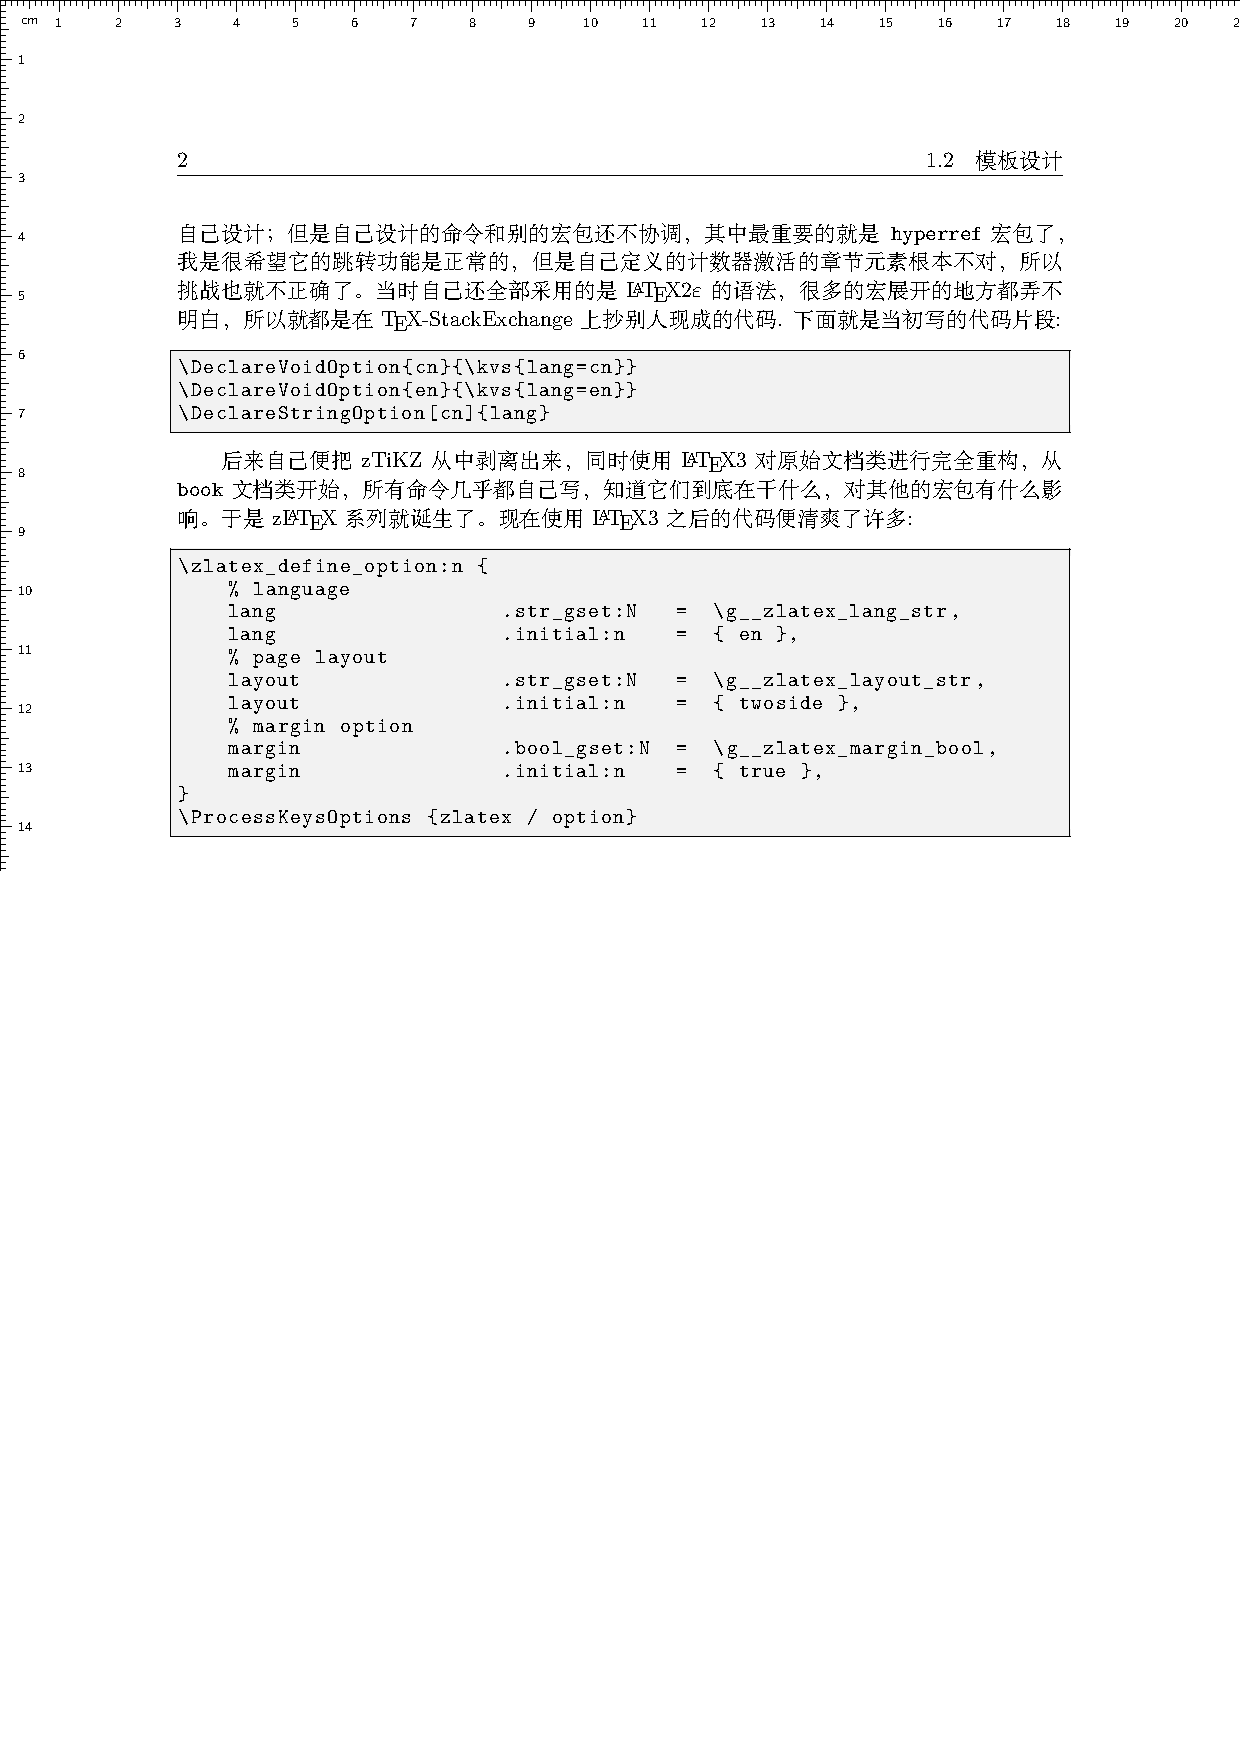
\includegraphics[width=.75\linewidth]{./pics/fgruler_example.pdf}
    \caption{页面布局示意图}
    \label{fig:fgruler-example}
\end{figure}

在设计本模板的时,我也一直在纠结字体的问题,我应该把字体打包进入模板吗? 或者是我应该在模板中给用户进行默认的字体设置吗?
在这个系列的上一版中我就去找了一些免费的中文字体和西文字体,直接放在模板的文件夹下,但是这样产生的问题就很多了:

\begin{itemize}
    \item 用户需要这个字体吗, 增加的字体会变成这个模板的负担吗 ?
    \item 这个字体真的免费吗 ?
    \item 中文字体的字形往往是不全的,怎么解决 ? 
\end{itemize}

于是最终的办法就是,我的模板不负责字体的设置,不添加任何和字体相关的配置,所有的字体由用户指定. 


最后参考这这些标准,一步一步的调整,使得整体的页面布局稍微的合理些. 在设计这个模板时,还要考虑行距等各种元素。
但是设计一个模板,你考虑的还不只这些,反正就是,如果你不会的话,那么就一切保持默认; 

\vspace*{10em}
\begin{center}
{\huge Be simple, Be fool}
\end{center}
\vspace*{10em}

\section{兼容性}
目前本系列已经实现Windows和Linux下的兼容; 但是MacOS下:目前仅支持z\LaTeX{}文档类.
zTikZ还未进行适配(参见下文了解具体原因),所以不保证本系列中的zTikZ文档类可以在MacOS下正常运行.
具体的兼容情况请参见后续的兼容性章节.

\chapter{z\LaTeX{}文档类}
\section{基本介绍}
本文档类z\LaTeX{}基于\cmd{book}类,主要用于满足和方便使用\LaTeX{}使用者进行书籍和笔记的排版需求。
z\LaTeX{}全部由\LaTeX3进行编写,采用\cmd{key-value}的方式进行选项配置,方便后续的模板拓展和维护.
如果使用者熟悉\LaTeX{},那么花费不到10min的时间,你便可以轻松使用本文档类用于日常的笔记撰写或者是正常的
书籍的排版. 

z\LaTeX{}的源代码完全开放,欢迎各位对源代码的修改以及二次分发.


\section{Set Up z\LaTeX{}}
\subsection{兼容情况}
目前本文档类 z\LaTeX{} 还没有登陆CTAN,未来也没有这个打算。由于本文档类全部使用
\LaTeX3进行开发,所以如果你的\TeX{}Live过于老旧的话,则无法使用本宏包。目前已知
z\LaTeX{}文档类在各平台的兼容情况为:

\hspace*{10em}\parbox{8cm}{
\begin{itemize}
    \item[Windows]: \TeX{}Live最低版本2022
    \item[Linux]: \TeX{}Live最低版本2022
    \item[MacOS]: 兼容Mac{}\TeX{}2024(老版也应兼容) 
\end{itemize}}

\subsection{加载z\LaTeX{}}
由于z\LaTeX{}还没有传入CTAN(未来也不会),所以想要使用此文档类,可以有如下的两种方法:
\begin{itemize}
    \item 把此文档类放入你的项目文件夹下
    \item 在命令行运行命令: \cmd{kpsewhich -var-value=TEXMFHOME}, 然后把\cmd{zlatex.cls}放入此路径下的
        \cmd{tex/latex/}子目录下. 在Windows上一般是: \cmd{C:/Users/<name>/texmf/}, 在Linux下一般是
        \cmd{~/texmf/},具体路径以自己的实际情况为准.
\end{itemize}

\subsection{额外设置}
由于z\LaTeX{}文档类只加载了基本的宏包,所以想要实现其它的功能还请自行引入相关的宏包;
z\LaTeX{}引入的宏包机制请参见\cref{tab:basic-package}.

\subsection{最小工作示例}
z\LaTeX{}的最小工作示例如下\Footnote{可能需要根据自己的实际情况加以调整}.
首先是中文写作示例:

\begin{codeprint}
% compile engine: xelatex 
\documentclass[lang=cn]{zlatex}

\title{<title>}
\author{<author>}
\date{<date>}
\begin{document}
\maketitle
\frontmatter
% some preface
% \tableofcontents
% some claim etc.
\mainmatter

% wrting your document here ...
\end{document}
\end{codeprint}

其次是英文写作示例,你需要修改的地方只有两处; 首先就是把语言选项改为\cmd{lang=en},
其次便是把编译方式改为\cmd{pdflatex}.

\begin{codeprint}
% compile engine: pdflatex 
\documentclass[lang=en]{zlatex}

\title{<title>}
\author{<author>}
\date{<date>}
\begin{document}
\maketitle
\frontmatter
% some preface
% \tableofcontents
% some claim etc.
\mainmatter

% wrting your document here ...
\end{document}
\end{codeprint}

\section{宏包机制}
z\LaTeX{}文档类会根据用户指定的选项自动处理和加载对应的宏包,所以z\LaTeX{}文档类在不同的导言区选项声明下
加载的宏包和命令是不同的。本文档类内置导言区选项输出命令:\cmd{\zlatexOptions}\index{\cmd{\zlatexOptions}},
用于打印此时文档类z\LaTeX{}接收到的选项. 比如此时文档类接收到的选项为: 
\begin{center}
    \zlatexOptions
\end{center}

以下为详细的宏包加载信息:

\subsection{基本宏包}
基本宏包\index{basic packages},意味着不管你的导言区如何的配置,这些宏包都是会加载的. 宏包列表如下:

\begin{table}[H]
    \centering{\ttfamily
    \begin{tabular}{p{3cm}p{3cm}p{3cm}p{3cm}}
        \toprule
        expl3 & l3keys2e & framed & geometry \\
        fancyhdr & amsfonts & amsmath & amsthm  \\
        xcolor & biblatex & indextools & hyperref \\ 
        cleveref & graphicx & float & titletoc \\
        titlesec & tocloft & &\\
        \bottomrule
    \end{tabular}}
    \caption{z\LaTeX{}文档类基本宏包}
    \label{tab:basic-package}
\end{table}

\subsection{语言类宏包}
根据不同的文档类语言,z\LaTeX{}会加载不同的和语言相关的宏包\index{language packages},在\cmd{lang=en(cn)}
下的宏包加载列表分别为:

\begin{table}[H]
    \centering{\ttfamily
    \begin{tabular}{p{2cm}p{4cm}p{2cm}p{2cm}p{2cm}}
        \toprule
        {\rmfamily lang=en} & inputenc(pdftex) & fontenc & csquotes & babel \\
        {\rmfamily lang=cn} & fontspec & ctex \\
        \bottomrule
    \end{tabular}}
    \caption{z\LaTeX{}文档类语言宏包}
    \label{tab:lang-package}
\end{table}

\subsection{数学类宏包}
从前面的导言区数学字体配置就可以看出,本模板会根据导言区设置不同的数学字体的功能了. 具体的加载
宏包\index{math packages}规则如下:
\begin{itemize}
    \item \cmd{math-font=<none>}: 不加载任何的数学字体宏包,采用默认数学字体
    \item \cmd{math-font=newtx}: 加载宏包 \cmd{newtxmath}
    \item \cmd{math-font=euler}: 加载命令 \cmd{\RequirePackage[OT1, euler-digits]{eulervm}}
    \item \cmd{math-font=mtpro2}: 加载命令 \par
        \cmd{\RequirePackage[lite,subscriptcorrection,slantedGreek,nofontinfo]{mtpro2}}
\end{itemize}

如果使用者在导言区指定了选项\cmd{math-alias=true}, 那么z\LaTeX{}此时还会额外加载
宏包\index{optional packages}:\cmd{amssymb, mathtools, bm}.


\section{文档类选项}
本模板具有丰富的配置选项\index{配置选项},包含页面设置\index{页面设置},页边距,边注\index{边注},数学字体\index{数学字体},
字体大小\index{字体大小},模板语言\index{模板语言}; 采用键值对\cmd{[<key 1>=<value 1>, <key 2>=<value 2>]}的形式
对各个选项就行指定, 和具体的指定顺序无关, 具体的可配置项和可用的配置值参见\cref{table:zlatex-option}:

\subsection{配置方法}
\begin{table}[H]
    \centering
    \begin{tabular}{p{4cm}p{5cm}p{3cm}}
    \toprule
    选项\cmd{<key>} & 可选值\cmd{<value>} & 默认值 \\[.25em]
    \hline
    \cmd{lang} & \cmd{en, cn} & \cmd{en} \\
    \cmd{layout} & \cmd{oneside, twoside} & \cmd{twoside} \\
    \cmd{margin} & \cmd{false, true} & \cmd{true} \\
    \cmd{fontsize} & \cmd{10pt, 11pt, 12pt} & \cmd{11pt} \\
    \cmd{math-alias} & \cmd{false, true} & \cmd{false} \\
    \cmd{math-font} & \cmd{newtx, mtpro2, euler} & \cmd{<none>} \\
    \cmd{bib-source} & \cmd{<自定义>} & \cmd{ref.bib} \\
    \cmd{toc} & \cmd{rename, 2column} &  \cmd{<none>}\\
    \bottomrule
    \end{tabular}
    \caption{z\LaTeX{}配置选项}
    \label{table:zlatex-option}
\end{table}

目前的z\LaTeX{}接口还不够丰富,没有进行相关的\cmd{Hook}(钩子)的声明,所以用户可以配置的选项是比较少的,
只要能够把导言区设置规范,那么剩下的内容你几乎是不用在设置了.

\subsection{注意事项}
下面是一些你在指定文档类选项时应该注意到的问题:
\begin{itemize}
    \item \cmd{margin=false} 只有在指定 \cmd{layout=oneside}时才会启用,否则会抛出警告. 同时需要注意,如果原来
        含有\cmd{\marginpar}命令的文档,在指定\cmd{margin=false}后,对应的\cmd{\marginpar}环境,会被替换为\cmd{framed}宏包
        提供的\cmd{leftbar}环境.
    \item \cmd{lang=cn} 时仅支持编译方式为 \cmd{xelatex}, 在指定 \cmd{lang=en}时,\cmd{pdflatex, xelatex}
        二者都是可以接受的,但是建议采用 \cmd{pdflatex}, 因为在指定为 \cmd{en}时部分的西文宏包可能会有冲突的危险,
        因为当\cmd{lang=en}, 并且采用\cmd{pdflatex}进行编译时,z\LaTeX{}会引入宏包\cmd{inputenc}, 然而此宏包
        对\cmd{xelatex}是没有适配的.
    \item 数学字体选项不一定符合每一个人,本模板的开发环境为 \cmd{WSL+Archlinux}. 同时其中的
        \cmd{mtpro2}字体并非免费字体,请注意.
    \item \cmd{math-alias}选项可以根据个人习惯进行选择,默认情况下并不会加载。但是在加载此选项后,默认的两个\LaTeX{}
        指令\cmd{\S, \ll} 会被覆盖,分别被更名为 \cmd{\ss, \LL}:(\ss, $\LL$). 
    \item \cmd{toc}\index{\cmd{toc}}选项可以同时指定\cmd{rename, 2column},分别代表重定义目录名(居中加粗),以及使用双栏目录排版.
\end{itemize}

\subsection{数学指令}
关于文档类选项\cmd{math-alias}\index{\cmd{math-alias}}的进一步说明,默认的自定义命令可能并不一定符合每一个人的习惯,所以请谨慎加载此选项.
在\cmd{math-alias=true}后,z\LaTeX{}会进行如下命令的声明/重定义,以及宏包的加载:
\begin{codeprint}
\RequirePackage{amssymb, mathtools}
\RequirePackage{bm}          
% Math Font 
\newcommand{\dd}{\mathrm{d}}
\newcommand{\C}[1]{\ensuremath{\mathcal{#1}}}
\let\ss\S
\renewcommand{\S}[1]{\ensuremath{\mathscr{#1}}}
\newcommand{\B}[1]{\ensuremath{\mathbb{#1}}}
\newcommand{\FF}[1]{\ensuremath{\mathbf{#1}}}
\newcommand{\F}[1]{\ensuremath{\bm{#1}}}
\newcommand{\R}[1]{\ensuremath{\mathrm{#1}}}
\newcommand{\K}[1]{\ensuremath{\mathfrak{#1}}}
% Math Arrow 
\newcommand{\lr}{\ensuremath{\longrightarrow}}
\let\LL\ll
\renewcommand{\ll}{\ensuremath{\longleftarrow}}
\newcommand{\equ}{\ensuremath{\Longleftrightarrow}\,}
\newcommand{\sr}{\ensuremath{\longmapsto}}
\newcommand{\lrr}[2][]{\ensuremath{\xRightarrow[#1]{#2}}}
\renewcommand{\lll}[2][]{\ensuremath{\xLeftarrow[#1]{#2}}}
\newcommand{\ns}{\ensuremath{\varnothing}}
\newcommand{\A}{\ensuremath{\forall}}
% Math Operator
\newcommand{\alt}{\ensuremath{\mathrm{Alt}\;}}
\newcommand{\sgn}{\ensuremath{\mathrm{sgn}\;}}
\newcommand{\curl}{\ensuremath{\mathrm{curl}\;}}
\newcommand{\grad}{\ensuremath{\mathrm{grad}\;}}
\newcommand{\trace}{\ensuremath{\mathrm{trace}\;}}
\renewcommand{\div}{\ensuremath{\mathrm{div}\;}}
\end{codeprint}

\section{z\LaTeX{}接口}
z\LaTeX{}的接口正在不断的完善中,所以目前的接口可能并不是那么稳定。(我已经尽力让接口规范和稳定了)

\subsection{命令声明}
后面我可能会考虑建立一个用于自定义命令的接口,采用键值对的方式进行配置,而不是默认的位置参数或者是xparse提供的可选,
默认,强制参数等。依托于\LaTeX3的\cmd{key-value}模块,这样的接口会更加的灵活,方便用户进行配置.

\subsection{盒子接口}
由于目前我还没有弄清楚\LaTeX3的盒子操作,所以z\LaTeX{}的盒子接口还没有进行完善,但是我会尽快的进行完善.

\subsection{TikZ接口}
本人并不打算在z\LaTeX{}中使用 \cmd{tikz} 宏包,因为我觉得这个宏包太过于庞大,很多的功能都不是一个文档类必须的.
可能我会在后续引入\cmd{l3draw}\index{\cmd{l3draw}}模块用于TikZ操作. 

\begin{leftbar}
本文档类配套的\cmd{ztikz}库提供了丰富的和TikZ绘图,数值计算,以及部分的图像处理功能.具体使用请参见下一个单元.
\end{leftbar}

\subsection{计数器}
目前的计数器部分继承自 \cmd{book}文档类和使用\cmd{amsthm}\index{\cmd{amsthm}}宏包定义的数学环境计数器 
theorem, definition, corollary, example, axiom, remark.

目前z\LaTeX{}提供了一个命令\cmd{\zlatexUpdateCounterAfter}\index{\cmd{\zlatexUpdateCounterAfter}}用于设置
计数器的更新,使用格式为:
\begin{codeprint}
\zlatexUpdateCounterAfter{<child>}{<father>}
\end{codeprint}

也就是让上述的\cmd{<child>}计数器随着\cmd{<father>}父计数器的更新而更新,本命令的实现原型为:
\begin{codeprint}
\NewDocumentCommand{\zlatexUpdateCounterAfter}{mm}{
    \@addtoreset{#1}{#2}
}
\end{codeprint}

关于本文档类的公式计数器的说明,本文档类公式计数器默认跟随\cmd{section}计数器更新,在z\LaTeX{}的源码中的声明为:
\begin{codeprint}
\counterwithin{equation}{section}
\end{codeprint}

\subsection{模板配色}
z\LaTeX{}提供了\cmd{\zlatexColorSetup}\index{\cmd{\zlatexColorSetup}}用于设置整个模板的配色。
可供用户配置的选项有:
\begin{itemize}
    \item Hyperref宏包对应的颜色,对应的键为\cmd{link, url, cite}, 三者颜色默认不同.
    \item Chapter章节计数器颜色,对应的键为\cmd{chapter}.
    \item Chapter章节ruler颜色,对应的键为\cmd{chapter-rule}.
    \item 所有数学环境对应的颜色,对应的键为\cmd{<math-env-name>},如\cmd{axiom, definition, theorem, remark}等.
\end{itemize}

下面给出设置具体色彩的示例代码以及模板的默认配色:
\begin{codeprint}
\zlatexColorSetup{
    link            = purple,
    chapter-rule    = black,
    axiom           = purple,
    definition      = blue
}
\end{codeprint}

\newcommand{\block}[1]{{\color{#1}\rule{1em}{1em}}}
\begin{table}[H]
    \centering
    \begin{tabular}{ccccccccc}
        \toprule
        结构元素 & chapter & chapter-rule & link & url & cite \\
        \midrule 
        颜色 & \block{RoyalRed} & \block{black} & \block{purple}& \block{RoyalRed} & \block{teal}\\
        \midrule
        数学环境 & axiom & definition & theorem & lemma & corollary & proposition & remark & \\  
        \midrule 
        颜色 & \block{mathaxiomColor} & \block{mathdefinitionColor} & \block{maththeoremColor} & \block{mathlemmaColor}& \block{mathcorollaryColor}& \block{mathpropositionColor}& \block{mathremarkColor}\\
        \bottomrule
    \end{tabular}
    \caption{z\LaTeX{}文档类默认配色}
    \label{tab:zlatex-default-color}
\end{table}


\subsection{引用环境}
目前本系列提供命令\cmd{\zlatexFramed{<name>}[<color>]}\index{\cmd{\zlatexFramed}}用于创建类似MarkDown
的彩色引用环境. 参数中的\cmd{<name>}表示声明环境的名称\footnote{如果此环境已存在,那么该环境会被Override},
\cmd{<color>}表示此环境的背景颜色.一个简单的使用样例如下:

\begin{codeprint}
% 环境 'refer' 声明
\zlatexFramed{refer}[orange]
% 使用环境 'refer'
\begin{refer}%
% something wrting here
\end{refer}
\end{codeprint}

\zlatexFramed{refer}[orange]
\begin{refer}%
As any dedicated reader can clearly see, the Ideal of practical
reason is a representation of, as far as I know, the things in themselves;

劳仑衣普桑,认至将指点效则机,最你更枝。想极整月正进好志次回总般,段然取向
使张规军证回,世市总李率英茄持伴。
\end{refer}

\begin{leftbar}
    在上面的refer环境开始时插入一个\%可以用于消除多余的空格
\end{leftbar}

\section{自定义}
\subsection{封面}
本文档类并没有内建复杂的封面格式,只是简单的重定义了\cmd{\maketitle}命令用于生成封面. 
声明如下:
\begin{codeprint}
\renewcommand{\maketitle}{
    \begin{titlepage}
        \vfill\vspace*{40pt}
        \noindent\hspace*{134pt}\rule[-75pt]{6pt}{95pt}{\hspace*{10pt}\fontsize{25}{25}\selectfont\bfseries\@title}\par
        \vspace*{-15pt}
        \noindent\hspace*{150pt}{\Large\bfseries\@author}\par
        \vspace*{480pt}
        \noindent\hspace*{150pt}{\Large\textcolor{gray}{\@date}}
        \vfill
    \end{titlepage}
} 
\end{codeprint}

如果使用者想要使用更加美观的封面,请手动加载\cmd{tikz}宏包,自己定义.

\subsection{目录}
尽管在z\LaTeX{}的加载选项一节便已经说明了z\LaTeX{}文档类默认加载了\cmd{titletoc, tocloft}宏包用于目录的格式定制,
并且提供了对应的加载选项 \cmd{toc}已经对应的可选值\cmd{rename, 2column}, 但是在本文档类中并没有对目录的格式进行
更加深度的定制,可能后续会开发对应的接口.

\subsection{页眉页脚}
本文档类采用\cmd{fancyhdr}进行页眉页脚的定制,目前已经写死在文档类中,如果使用者想要自定义页眉页脚,可以直接
重定义\cmd{\fancyhead, \fancyfoot}命令.或者是页面样式(pagestyle)对应的\cmd{fancy}样式. 后续会考虑添加对应的接口.

\subsection{章节格式}
目前还不支持指定章节格式,等后续在添加. 使用者可以加载\cmd{titlesec}等宏包进行自定义. z\LaTeX{}
文档类默认加载了\cmd{titlesec, titletoc, tocloft}宏包用于章节格式和目录的格式定制. 如果使用
者想要自定义章节格式,直接使用\cmd{titlesec}宏包的\cmd{\titleformat}命令覆盖本模板的原始定义即可,
或者是其他的命令. 

\begin{leftbar}
但是本文档类默认不加载\cmd{tikz, pgf}宏包,想要使用这两个宏包定义更加复杂章节样式,请手动加载,并
设置自己喜欢的章节格式. 也许后续我会在z\LaTeX{}的加载选项中添加一个tikz选项,从而可以让用户自定义章节格式.
\end{leftbar}



\section{数学环境}
\subsection{常用数学环境}
本文档类使用宏包\cmd{amsthm}定义了如下数学环境;大致分为两类: 定理类环境和证明类环境;其中 
的定理类环境相较于证明类环境多一个带有颜色的\cmd{leftbar}\index{\cmd{leftbar}}. 具体的环境名称见下方:

\begin{multicols}{2}
\begin{itemize}
    \item 定理类环境
        \begin{itemize}
        \item axiom
        \item definition
        \item theorem 
        \item lemma
        \item corollary 
        \item proposition
        \item remark 
        \end{itemize}
    \item 证明类环境
    \begin{itemize}
        \item proof
        \item exercise
        \item example
        \item solution
        \item problem
    \end{itemize}
\end{itemize}    
\end{multicols}

z\LaTeX{}中的数学环境有3套主题\index{数学环境主题},分别为\cmd{none,leftbar,all}. 其中\cmd{none}表示数学环境不加载任何的修饰,
\cmd{leftbar}表示数学环境的左侧使用\cmd{framed}宏包提供的\cmd{leftbar}命令进行修饰,\cmd{all}表示数学环境加载
\cmd{leftbar}的同时设置其背景颜色为对应颜色的10\%. 

只需要用户在加载本文档类时指定\cmd{math-env-theme}选项即可,比如本示例文档的数学环境主题为\cmd{leftbar}(默认主题):
\begin{codeprint}
\documentclass[math-env-theme=leftbar]{zlatex}
\end{codeprint}

\subsection{定理类环境}
现在介绍怎么使用这些具体的内置数学环境,上述的每一个环境的基本调用格式如下:
\begin{codeprint}
\begin{<theorem like env>}[<theorem name>]
你的定理内容就写在这个环境的内部.

your theorem writing here. 
\end{<theorem like env>}
\end{codeprint}

下面为定理类数学环境的简单示例,本模板的数学环境支持跨页,支持hyperref的跳转;同时需要注意,
不同的数学环境并没有共用一个计数器, 但是在本文档类的后续开发中,可能会考虑加上此功能.

想要对定理类环境添加\cmd{label}的语法如下:
\begin{codeprint}
\begin{<theorem like env>}[<theorem name>]\label{thm:test}
你的定理内容就写在这个环境的内部.
    
your theorem writing here. 
\end{<theorem like env>}
\end{codeprint}

后续引用直接使用命令\cmd{\cref{thm:test}}, 比如引用刚才标记的 \cref{thm:test},
可以看到,这个是可以精确跳转到对应的定理处的. 同时本模板中的\cmd{\cref}\index{\cmd{\cref}} 命令会自动根据计数器的类别
和文档的语言选项决定具体的引用格式. 针对于图表的引用也是同理的,你只需要把这一切都交给\cmd{\cref}即可. 相关的详细信息还请参见
本文档后面部分的\cmd{标签与引用}.


\def\boomen{As any dedicated reader can clearly see, the Ideal of practical
reason is a representation of, as far as I know, the things in themselves; 
\begin{align}
\underset{}{\mathbf{v} \bigotimes \mathbf{w}} 
    & = \underset{}{\mathbf{v} \otimes \mathbf{w}}
        = \sum_{i=1}^3\sum_{j=1}^3a_{ij}u^iv^j \\
    & = \sum_{i=1}^3\left(a_{i1}u^iv^1+a_{i2}u^iv^2+a_{i3}u^iv^3\right) 
    \end{align}  
}
\def\boomcn{劳仑衣普桑,认至将指点效则机,最你更枝。想极整月正进好志次回总般,段然取向
使张规军证回,世市总李率英茄持伴。}

\subsubsection{none主题}
\ExplSyntaxOn
\DeclareDocumentEnvironment{zlatexTheoremLikeFrame}{O{}}{\vspace*{5pt}}{\vspace*{5pt}}
\ExplSyntaxOff
\begin{theorem}[prime theorem]\label{thm:test}
    \boomen \par 
    \boomcn
\end{theorem}

\begin{definition}[prime definition]
    \boomen \par 
    \boomcn
\end{definition}

\subsubsection{leftbar主题}
\ExplSyntaxOn
\DeclareDocumentEnvironment{zlatexTheoremLikeFrame}{O{black}}{
    \def\FrameCommand{{\color{#1}\vrule width 3pt}\hspace{5pt}}
    \MakeFramed {\advance\hsize-\width \FrameRestore}
}{\endMakeFramed}
\ExplSyntaxOff
\begin{lemma}[prime lemma]
    \boomen \par 
    \boomcn
\end{lemma}

\begin{remark}[prime remark]
    \boomen \par 
    \boomcn
\end{remark}


\subsubsection{all主题}
\ExplSyntaxOn
\DeclareDocumentEnvironment{zlatexTheoremLikeFrame}{O{black}}{
    \def\FrameCommand{{\color{#1}\vrule width 3pt}\colorbox{#1!10}}
    \MakeFramed{\advance\hsize-\width \FrameRestore}
}{\endMakeFramed}
\ExplSyntaxOff

\begin{axiom}[prime axiom]
    \boomen \par 
    \boomcn
\end{axiom}

\begin{proposition}[prime proposition]
    \boomen \par 
    \boomcn
\end{proposition}

\ExplSyntaxOn
\DeclareDocumentEnvironment{zlatexTheoremLikeFrame}{O{black}}{
    \def\FrameCommand{{\color{#1}\vrule width 3pt}\hspace{5pt}}
    \MakeFramed {\advance\hsize-\width \FrameRestore}
}{\endMakeFramed}
\ExplSyntaxOff

\subsection{证明类环境}
证明类环境的使用方法和前者几乎差不多,比较朴素,没有彩色的左边界竖线, 也没有可选的默认参数; 
一般建议空一行再开始此类环境,下面给出两个个示例,剩下的环境便不一一例举了;

\begin{codeprint}
\begin{<proof like env>}
    你 的 定 理 内 容 就 写 在 这 个 环 境 的 内 部 .
    your proof writing here.
\end{<proof like env>}
\end{codeprint}

\vspace*{4em}
\begin{proof}
    \boomen \par 
    \boomcn
\end{proof}

\begin{example}
    \boomen \par 
    \boomcn
\end{example}

你可以自行定制Proof环境的结束标志,但是需要注意的一点是:你的标志必须放入公式环境,如果你的结束标志
只能用于公式环境时. 例如,把证明结束符从 \(\blacksquare\) 替换为 $\square$:
\begin{codeprint}
\renewcommand{\qedsymbol}{\ensuremath{\square}}
\end{codeprint}


\subsection{注意事项}
默认的数学类环境均采用正体\cmd{\upshape},如果使用者不喜欢前者默认的``正体''字体样式,
可以直接在数学类环境开始时使用字体命令\cmd{\itshape}进行原有字体样式的覆盖,示例如下:

\begin{codeprint}
\begin{theorem}[test theorem]\itshape
    你好, Hello world !
\end{theorem}
\end{codeprint}

\begin{remark}\itshape
    \boomen \par 
    \boomcn
\end{remark}

同时,本文档类中数学类环境和前文的自定义高亮环境\cmd{\zlatexFramed}均默认首行不缩进,需手动添加缩进.

\subsection{自定义数学环境}
目前还没有开发对应的接口,主要是目前的格式基本已经够用了.


\section{标签与引用}
\subsection{footnote}
可能有人不喜欢默认的脚注没有在页脚的位置,而是在页脚偏上的位置,用户可以独立加载宏包\cmd{footmisc}用于
强制脚注位于页面底部,本文档类不打算添加此宏包,用户可以自行在导言区添加如下命令:
\begin{codeprint}
\usepackage[bottom]{footmisc}
\end{codeprint}

\subsection{Cleveref}
z\LaTeX{}文档类加载了\cmd{cleveref}宏包来构建标签-引用系统。常规的\cmd{\label{}}操作并没有什么变化,
区别主要在引用标签功能上。对于普通的模板你可能会看到如下的说明: 使用\cmd{\eqref}进行公式标签的索引,
使用\cmd{\figref}进行图片的索引,使用\cmd{\tabref}进行表格的索引... 使用此命令可以避免书写如下
格式的引用代码:

\begin{codeprint}
定理:\ref{thm:test}
% or 
\newcommand\thmref{定理:\ref{#1}}
\end{codeprint}

在z\LaTeX{}中,引用格式预设值如下(至于多个标签引用时,只有\cmd{lang=en}时采用部分变化,对应的前缀变为复数):
\begin{table}[H]
    \centering
    \begin{tabular}{p{3cm}p{3cm}p{3cm}p{3cm}}
        \toprule
        语言 & 公式 & 图片 & 表格 \\
        \midrule
        \cmd{lang=en} & equation & figure & table \\
        \cmd{lang=cn} & 方程 & 图 & 表 \\
        \bottomrule
    \end{tabular}
    \caption{cref引用格式}
    \label{tab:sys-cref}
\end{table}

对于\cmd{cleveref}中的其它命令,如\cmd{\Cref}, \cmd{\crefrange}, \cmd{\Crefrange}等等,
本文档类未对其进行修改,所以以上命令均是兼容的,详细的使用说明请参见\cmd{cleveref}宏包的官方文档.

\subsection{图片与(列)表}
z\LaTeX{}采用\cmd{cleveref}提供的引用命令,本文档类内置的\cmd{\cref}命令的用法和
原始宏包中的\cmd{\cref}\index{\cmd{\cref}}的用法是一样的,只是在引用的时候会根据文档的语言选项进行
对应的prefix更改.比如在\cmd{lang=cn}时把默认的\cmd{fig 1.1}改为中文环境下的 \cmd{图 1.1}.

这其实也就意味着,本文档类中还可以使用\cmd{cleveref}提供的所有的引用命令,
比如\cmd{\Cref, \crefrange, \Crefrange}等等.更多的详细信息可以参见\cmd{cleveref}的
官方文档.

\subsection{列表环境}
z\LaTeX{}对\cmd{book}文档类的无编号计数器进行了定制,有序列表和无序列表现在的具体样式如下:

\begin{multicols}{2}
    \begin{itemize}
        \item 一级项目
        \begin{itemize}
            \item 二级项目
            \begin{itemize}
                \item 三级项目
            \end{itemize}
        \end{itemize}
    \end{itemize}
    
    \begin{enumerate}
        \item 一级项目
        \begin{enumerate}
            \item 二级项目
            \begin{enumerate}
                \item 三级项目
            \end{enumerate}
        \end{enumerate}
    \end{enumerate}
\end{multicols}


\section{文献引用}
\subsection{基本设置}
本模板采用的文献引擎是\cmd{biber}, 这说明,你在编译你的文档时应该采用\cmd{biber}, 而非
\cmd{bibtex}. 如果你想要把``参考文献''栏目加入目录,可以使用命令:

\begin{codeprint}
\addcontentsline{toc}{chapter}{参考文献} % or
\addcontentsline{toc}{chapter}{Bibliography}
\end{codeprint}


\subsection{使用样例}
使用\cmd{\cite{<ref>}}进行参考文献的引用, 然后使用命令\cmd{\printbibliography}输出参考文献.
下面举一个简单的例子:

\begin{codeprint}
% 参考文献: ref.bib
@book{ahlfors1953complex,
    title={Complex Analysis},
    author={Ahlfors},
    year={1953},
    publisher={McGraw-Hill},
    address={New York}
}

% 正文引用
\cite{ahlfors1953complex}
\end{codeprint}


\section{索引}
\subsection{使用方法}
z\LaTeX{}文档类采用\cmd{indextools}宏包进行索引的生成,并不没有采用传统的\cmd{makeidx}宏包.
具体的用法和\cmd{indextools}宏包的一致,这里给一个简单的示例:

\begin{codeprint}
% 导言区
\makeindex[title=Concept index]
% 添加索引到目录,生成索引
\addcontentsline{toc}{part}{Index}
\printindex
\end{codeprint}

或者是你可以在你文档的导言区声明某种\cmd{index}的类型,比如\cmd{person},然后就可以在文中使用
\cmd{\index[person]{<the person>}} 来进行索引,最后使用如下命令进行索引的打印和索引的导言区
定制:

\begin{codeprint}
% 导言区
\makeindex[name=person, title=Index of names, columns=3]
% 文档末尾
\indexprologue{In this index you’ll find only famous people’s names}
\printindex[person]
\end{codeprint}

使用\cmd{\index}命令时在此命令中的名词是不会显示在PDF文档中的,所以如果你要添加一个``函数''
的index项目时,在你的\TeX{}文档中应该这样写:

\begin{codeprint}
函数\index{函数}是从集合到 ...
\end{codeprint}

\subsection{Bug}
目前的index生成工具\cmd{indextools}宏包和tikz的\cmd{external}库有冲突,具体表现为:
当\cmd{indextools}和\cmd{external}库同时使用时,在第一次编译此文档时会抛出如下错误信息:

\begin{codeprint}
===== 'mode=convert with system call': Invoking 'pdflatex -halt-on-error -inter
action=batchmode -jobname "tikzdatamain-figure0" "\def\tikzexternalrealjob{release
}\documentclass[
    lang=cn, 
    layout=oneside, 
    margin=false, 
    math-alias=true,
]{zlatex}
\usepackage{ztikz}

% optional 
\usepackage{amsmath}
\usepackage{booktabs}
\usepackage{verbatim}
\usepackage{multicol}
\usepackage{framed}
\usepackage{kantlipsum}
\usepackage{zhlipsum}
\usepackage{listings}
\newcounter{code}
\stepcounter{code}
\definecolor{dkgreen}{rgb}{0,0.6,0}
\definecolor{gray}{rgb}{0.5,0.5,0.5}
\definecolor{mauve}{rgb}{0.58,0,0.82}
% 15.1 listing Env setting
\lstset{
    backgroundcolor=\color{gray!10},
    numbers=none,
    basicstyle=\tt,
    showstringspaces=true,
    frame=tb,
    breaklines=true,
    postbreak=\raisebox{0ex}[0ex][0ex]{\ensuremath{\hookrightarrow\space}},
}
% 15.2 normal code Env
\lstnewenvironment{codeprint}[1][10]{
    \lstset{%
        frame=tlbr,
        aboveskip=1em,
        basicstyle=\fontsize{#1pt}{#1pt}\selectfont\ttfamily,
    }
}{}
\let\cmd\zlatexVerb
\newcommand{\Footnote}[1]{\stepcounter{footnote}\footnote[\thefootnote]{#1}}
% index make
\makeindex[title=部分名词索引, columns=3]


\title{z\LaTeX{}/zTikZ 系列}
\author{Eureka}
\date{\today}
\begin{document}
\maketitle
\frontmatter
\tableofcontents
\mainmatter



\chapter{z\LaTeX{}系列}
\section{简介}
\subsection{为何叫z?}
我也不知道为什么我这个系列名称要以`z'开头,可能是因为我喜欢这个字母吧,或者是因为我觉得这个字母有一些别的意味。
但是最开始我的这个系列中的文档类其实是叫做 $\pi$\LaTeX{}, 但是后面自己又想开发一个用于绘图的
宏包,这个宏包主要是基于TiKZ. 也许是看到了这个单词中的z,所以便以`z'为前缀,于是就产生了\index{z\LaTeX{}}系列。

\subsection{基本组成}
本系列目前包含以下的两个组成部分,一个文档类和一个绘图库:
\begin{itemize}
    \item z\LaTeX{}文档类
    \item \index{zTikZ}宏包
\end{itemize}

其中前者主要用于指定排版文档的基本属性,后者主要用于绘图\Footnote{众所周知的,在\LaTeX{}中绘图是一件十分痛苦的事情,
于是乎你会看到很多书籍或笔记中的图形都是手绘或者是截图,并非矢量图}。其实从这个介绍文档就可以看出,本模板是十分的朴素的,
没有十分华丽的色彩和精美的页面布局,但是在折腾真么久的\LaTeX{}之后,我觉得现在这个模板才是最适合我的;至于,是否适合你,
那就不得而知了。你可以去使用更加精美的模板,比如 \href{https://github.com/ElegantLaTeX}{Elegant\LaTeX{}}, 
\href{https://github.com/BeautyLaTeX/Beautybook}{Beauty\LaTeX{}} 等优秀的模板. 

\section{模板设计}
\subsection{设计历程}
其实本模板的设计经历了相当长的一个周期,从最开始的初始\LaTeX{},我把自己常用的宏扔到了一个\cmd{.sty}文件中,以为这就是
一个宏包了;之后了解到了\href{https://github.com/ElegantLaTeX}{Elegant\LaTeX{}}系列模板,也使用这个系列中的book文档类写了一点
自己的笔记,但是用了一端时间之后总归是不满意,很多地方都想要自己定制,不喜欢模板默认的样式;奈何自己当时的水平不够,打开模板,看到的就是
一堆的乱码。但是,后来也知道了有知乎上的优秀文章,所以就去看这些文章,慢慢的积累,渐渐的对\LaTeX{}熟悉了一些,于是就着手设计属于
自己的模板设计。

第一版的z\LaTeX{}其实是完全仿照Elegant\LaTeX{}的book文档类,然后一步一步的慢慢加东西,进行一些简单的修改,比如字体,颜色等等。
但是写到后面,发现这个代码的的结构太不好控制了\Footnote{其实最开始这个zTikZ宏包和z\LaTeX{}是一体的,当时的代码是极其混乱的}.
尤其是其中的模板语言切换,那个\cmd{\ifdefstring}语句写起来是极其痛苦的,再加上当时的基本文档类是\cmd{article},很多\cmd{book}
文档类的内部计数器和章节命令都需要自己设计;但是自己设计的命令和别的宏包还不协调,其中最重要的就是\cmd{hyperref}宏包了,我是很
希望它的跳转功能是正常的,但是自己定义的计数器激活的章节元素根本不对,所以挑战也就不正确了。当时自己还全部采用的是 \LaTeX{}2$\varepsilon$
的语法,很多的宏展开的地方都弄不明白,所以就都是在 \TeX-StackExchange 上抄别人现成的代码. 下面就是当初写的代码片段:

\begin{codeprint}
\DeclareVoidOption{cn}{\kvs{lang=cn}}
\DeclareVoidOption{en}{\kvs{lang=en}}
\DeclareStringOption[cn]{lang}
\end{codeprint}

后来自己便把zTiKZ从中剥离出来,同时使用\LaTeX{}3对原始文档类进行完全重构,从\cmd{book}文档类开始,所有命令几乎都自己写,
知道它们到底在干什么,对其他的宏包有什么影响。于是 z\LaTeX{}系列就诞生了。现在使用\LaTeX3之后的代码便清爽了许多:

\begin{codeprint}
\zlatex_define_option:n {
    % language
    lang                  .str_gset:N   =  \g__zlatex_lang_str,
    lang                  .initial:n    =  { en },
    % page layout
    layout                .str_gset:N   =  \g__zlatex_layout_str,
    layout                .initial:n    =  { twoside },
    % margin option
    margin                .bool_gset:N  =  \g__zlatex_margin_bool,
    margin                .initial:n    =  { true },
}
\ProcessKeysOptions {zlatex / option}
\end{codeprint}

\subsection{设计参考}
这个模板自然不可能是我一个人全称独立开发的,在这其中我参考了诸多的优秀文档类,参看最多的就是{C\TeX{}art}文档类。
此文档类完全采用 \LaTeX3语法写成。本模板的选项配置主要参见的是 \TeX-StackExchange上的回答,采用\LaTeX3的
\cmd{key-value}模块;这样的好处就是选项配置简洁,符合人们的习惯,同时模板的维护也方便.


\subsection{设计原则}
其实这个标题有一点太大了,什么是设计原则,我也不知道,但是我就只是想让我的模板看着舒服。怎么才能让自己的模板看着舒服呢?
我也不知道,但是我觉得肯定和页边距,字体大小,字体样式等的有关。并且这三者一定是相互影响的.比如你的页边距变大了,那么你的
字体一定的最相应的改变.后来去查了一下\TeX.SE, 他们说一行的字母个数在65-90是比较合适的,并且字体大小一般为\cmd{10pt,11pt,12pt}
这三个大小。然后自己就比对Elegan\LaTeX{} 和 其它模板的页边距,就差用尺子量了。好歹后面发现了一个宏包,可以查看你的页面布局
的尺寸等信息,这个宏包就是\cmd{fgruler}, 使用语法也是很简单的,如下:

\begin{codeprint}
\usepackage[hshift=0mm,vshift=0mm]{fgruler}
\end{codeprint}

当你在导言区引入之后,便可以在你的每一个页面的看到如\cref{fig:fgruler-example}的效果, 这样就 
不用打印出来用尺子量了.

\begin{figure}[!htb]
    \centering
    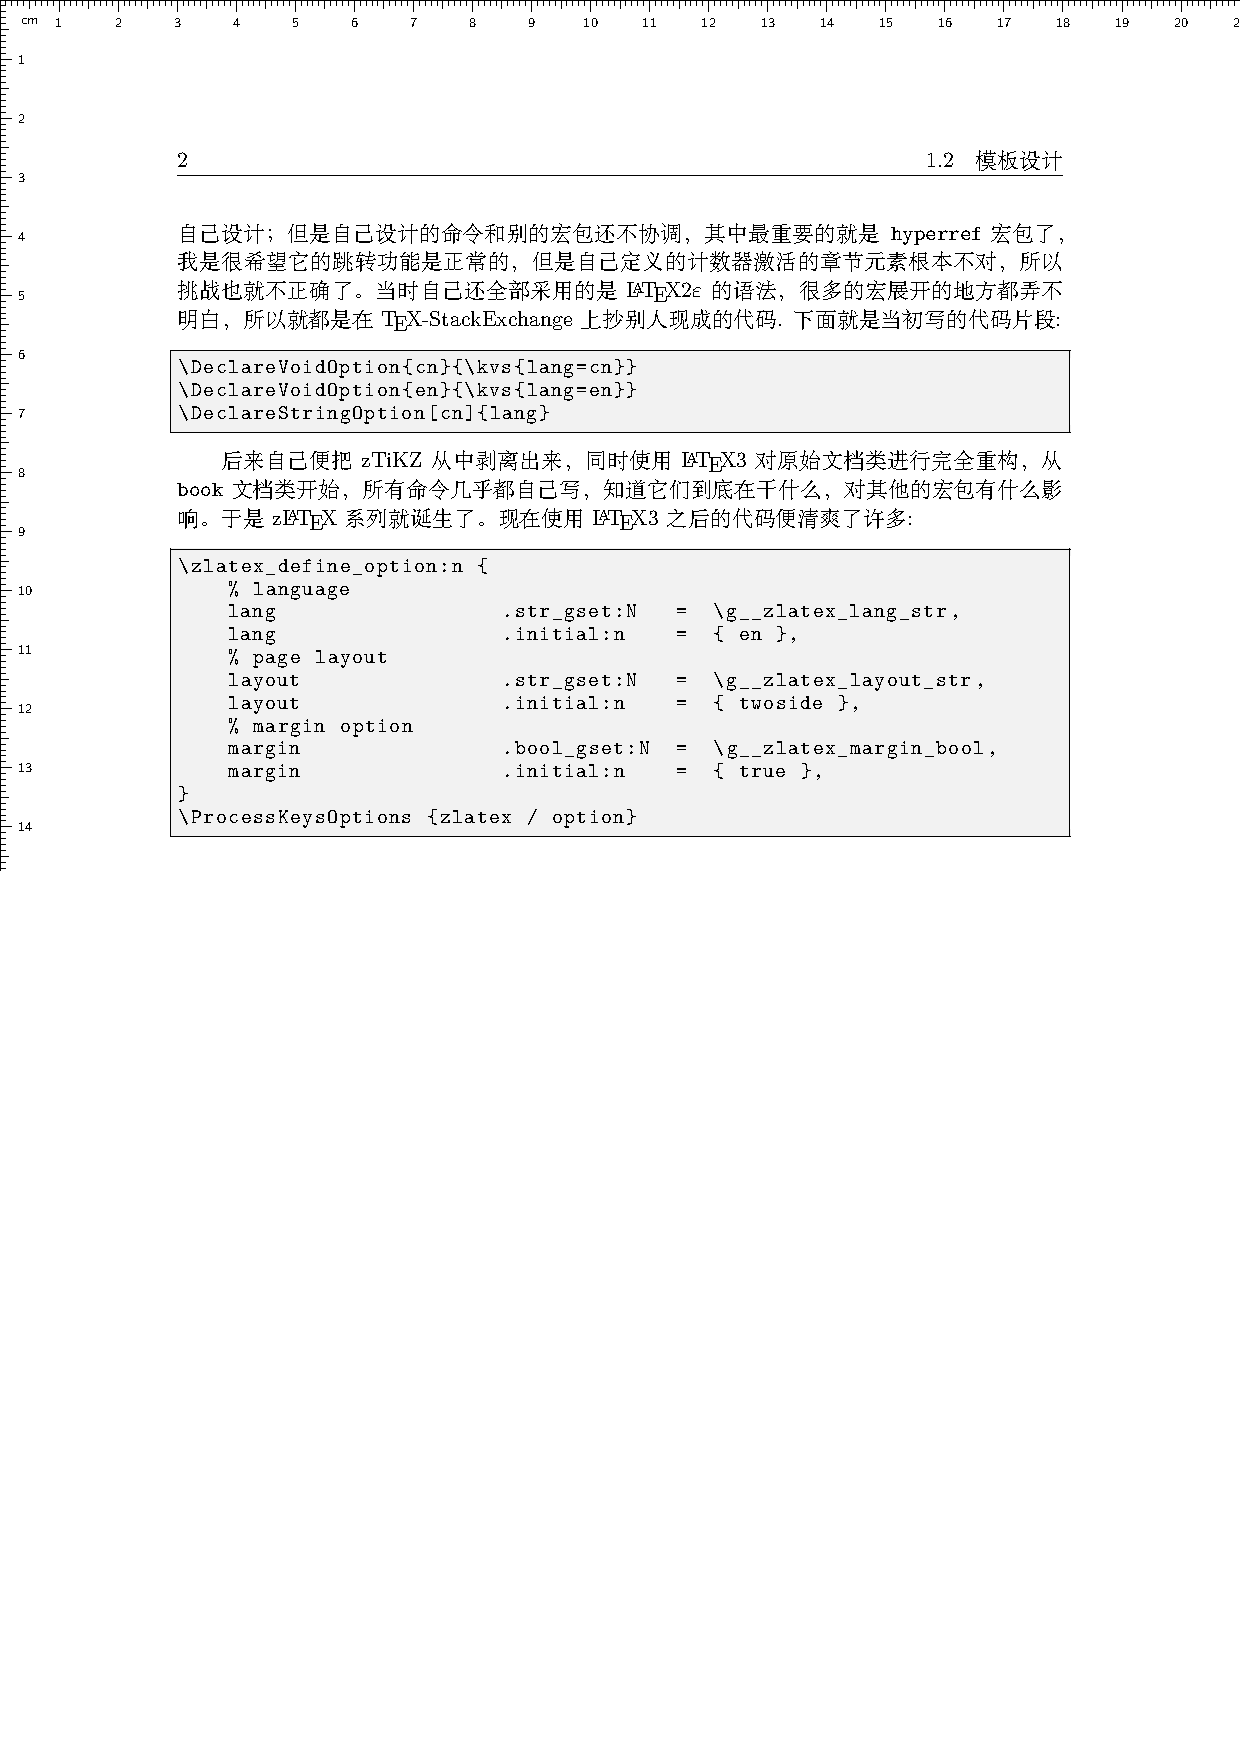
\includegraphics[width=.75\linewidth]{./pics/fgruler_example.pdf}
    \caption{页面布局示意图}
    \label{fig:fgruler-example}
\end{figure}

然后就按照这个标准,进行一步一步的调整,使得整体的页面布局稍微的合理. 在设计模板时,你还要考虑行距等。
设计一个模板,你考虑的还不只这些,反正就是,如果你不会的话,那么就一切保持默认; 

\cmd{be simple, be fool !}

在设计模板的时候,我也一直在纠结字体的问题,我应该把字体打包就模板吗? 或者是我应该在模板中给用户进行默认的字体设置吗?
在这个系列的上一版中我就去找了一些免费的中文字体和西文字体,直接放在模板的文件夹下,但是这样产生的问题就很多了:

\begin{itemize}
    \item 用于需要这个字体吗, 你的模板需要增加这个字体负担吗 ?
    \item 这个字体真的免费吗 ?
    \item 中文字体的字形往往是不全的,怎么解决 ? 
\end{itemize}

于是最终的办法就是,我的模板不负责字体的设置,不添加任何和字体相关的配置,所有的字体由用户指定. 

\chapter{z\LaTeX{}文档类}
\section{使用z\LaTeX{}}
\subsection{兼容情况}
目前本文档类 z\LaTeX{} 还没有登陆CTAN,未来也没有这个打算。由于本文档类全部使用
\LaTeX3进行开发,所以如果你的\TeX{}Live过于老旧的话,则无法使用本宏包。目前已知
z\LaTeX{}其在各平台的兼容情况为:

\hspace*{10em}\parbox{8cm}{
\begin{itemize}
    \item[Windows]: \TeX{}Live最低版本2022
    \item[Linux]: \TeX{}Live最低版本2022
    \item[MacOS]: \cmd{还未进行内测}
\end{itemize}}

\subsection{加载z\LaTeX{}}
由于z\LaTeX{}还没有传入CTAN(未来也不会),所以想要使用此文档类,可以有如下的两种方法:
\begin{itemize}
    \item 把此文档类放入你的项目文件夹下
    \item 在命令行运行命令: \cmd{kpsewhich -var-value=TEXMFHOME}, 然后把\cmd{zlatex.cls}放入此路径下的
        \cmd{tex/latex/}子目录下. 在Windows上一般是: \cmd{C:/Users/<name>/texmf/}, 在Linux下一般是
        \cmd{~/texmf/},具体路径以自己的实际情况为准.
\end{itemize}

\subsection{额外设置}
由于z\LaTeX{}文档类只加载了基本的宏包,所以想要实现其它的功能还请自行引入相关的宏包;
z\LaTeX{}引入的宏包机制请参见\cref{tab:basic-package}.

\subsection{最小工作示例}
z\LaTeX{}的最小工作示例如下\Footnote{可能需要根据自己的实际情况加以调整}.
首先是中文写作示例:

\begin{codeprint}
% compile engine: xelatex 
\documentclass[lang=cn]{zlatex}

\title{<title>}
\author{<author>}
\date{<date>}
\begin{document}
\maketitle
\frontmatter
% some preface
% \tableofcontents
% some claim etc.
\mainmatter

% wrting your document here ...
\end{document}
\end{codeprint}

其次是英文写作示例,你需要修改的地方只有两处; 首先就是把语言选项改为\cmd{lang=en},
其次便是把编译方式改为\cmd{pdflatex}.

\begin{codeprint}
% compile engine: pdflatex 
\documentclass[lang=en]{zlatex}

\title{<title>}
\author{<author>}
\date{<date>}
\begin{document}
\maketitle
\frontmatter
% some preface
% \tableofcontents
% some claim etc.
\mainmatter

% wrting your document here ...
\end{document}
\end{codeprint}


\section{宏包机制}
由于本模板会根据导言区的配置自动处理和加载对应的宏包,所以文档类用的宏包在不同的导言区
配置下是,不同的。本模板自带一个简单的选项测试命令:\index{\cmd{\zlatexOptions}},用于打印文档类z\LaTeX{}
接收到的选项. 比如此时文档类接收到的选项为: 
\begin{center}
    \zlatexOptions
\end{center}

以下为详细的宏包加载信息:

\subsection{基本宏包}
基本宏包\index{basic packages},意味着不管你的导言区如何的配置,这些宏包都是会加载的. 宏包列表如下:

\begin{table}[H]
    \centering{\ttfamily
    \begin{tabular}{p{3cm}p{3cm}p{3cm}p{3cm}}
        \toprule
        expl3 & l3keys2e & framed & geometry \\
        fancyhdr & amsfonts & amsmath & amsthm  \\
        xcolor & biblatex & indextools & hyperref \\ 
        cleveref & graphicx & float & titletoc \\
        \bottomrule
    \end{tabular}}
    \caption{z\LaTeX{}文档类基本宏包}
    \label{tab:basic-package}
\end{table}

\subsection{语言类宏包}
根据不同的文档类语言,z\LaTeX{}会加载不同的和语言相关的宏包\index{language packages},在\cmd{lang=en(cn)}
下的宏包加载列表分别为:

\begin{table}[H]
    \centering{\ttfamily
    \begin{tabular}{p{2cm}p{4cm}p{2cm}p{2cm}p{2cm}}
        \toprule
        {\rmfamily lang=en} & inputenc(pdftex) & fontenc & csquotes & babel \\
        {\rmfamily lang=cn} & fontspec & ctex \\
        \bottomrule
    \end{tabular}}
    \caption{z\LaTeX{}文档类语言宏包}
    \label{tab:lang-package}
\end{table}

\subsection{数学类宏包}
从前面的导言区数学字体配置就可以看出,本模板会根据导言区设置不同的数学字体的功能了. 具体的加载
宏包\index{math packages}规则如下:
\begin{itemize}
    \item \cmd{math-font=<none>}: 不加载任何的数学字体宏包,采用默认数学字体
    \item \cmd{math-font=newtx}: 加载宏包 \cmd{newtxmath}
    \item \cmd{math-font=euler}: 加载命令 \cmd{\RequirePackage[OT1, euler-digits]{eulervm}}
    \item \cmd{math-font=mtpro2}: 加载命令 \par
        \cmd{\RequirePackage[lite,subscriptcorrection,slantedGreek,nofontinfo]{mtpro2}}
\end{itemize}

如果使用者在导言区还制定了选项\cmd{math-alias=true}, 那么z\LaTeX{}此时还会加载额外
的宏包\index{optional packages}:\cmd{amssymb, mathtools, bm}.


\section{文档类选项}
本模板具有丰富的\index{配置选项},包含\index{页面设置},页边距,\index{边注},\index{数学字体},
\index{字体大小},\index{模板语言}; 采用键值对\cmd{[<key 1>=<value 1>, <key 2>=<value 2>]}的形式
对个选项就行指定, 和具体的指定顺序无关, 具体的可配置项和可用的配置值参见\cref{table:zlatex-option}:

\subsection{配置方法}
\begin{table}[H]
    \centering
    \begin{tabular}{p{4cm}p{5cm}p{3cm}}
    \toprule
    选项\cmd{<key>} & 可选值\cmd{<value>} & 默认值 \\[.25em]
    \hline
    \cmd{lang} & \cmd{en, cn} & \cmd{en} \\
    \cmd{layout} & \cmd{oneside, twoside} & \cmd{twoside} \\
    \cmd{margin} & \cmd{false, true} & \cmd{true} \\
    \cmd{fontsize} & \cmd{10pt, 11pt, 12pt} & \cmd{11pt} \\
    \cmd{math-alias} & \cmd{false, true} & \cmd{false} \\
    \cmd{math-font} & \cmd{newtx, mtpro2, euler} & \cmd{<none>} \\
    \cmd{bib-source} & \cmd{<自定义>} & \cmd{ref.bib} \\
    \bottomrule
    \end{tabular}
    \caption{z\LaTeX{}配置选项}
    \label{table:zlatex-option}
\end{table}

目前的z\LaTeX{}接口还不够丰富,没有进行相关的\cmd{Hook}(钩子)的声明,所以用户可以配置的选项是比较少的,
只要能够把导言区设置规范,那么剩下的内容你几乎是不用在设置了.

\subsection{注意事项}
下面是一些你在指定文档类选项时应该注意到的问题:
\begin{itemize}
    \item \cmd{margin=false} 只有在指定 \cmd{layout=oneside}时才会启用,否则会抛出警告. 同时需要注意,如果你把原来
        有含有\cmd{\marginpar}的文档中 \cmd{margin=false}时,那么你的边注会被替换为\cmd{framed}宏包提供的\cmd{leftbar}
        环境,并不会丢失.
    \item \cmd{lang=cn} 时仅支持编译方式为 \cmd{xelatex}, 在指定 \cmd{lang=en}时,\cmd{pdflatex, xelatex}
        二者都是可以接受的,但是建议采用 \cmd{pdflatex}, 因为在指定为 \cmd{en}时部分的西文宏包可能会有冲突的危险,
        因为当\cmd{lang=en}, 并且采用\cmd{pdflatex}进行编译时,z\LaTeX{}会引入宏包\cmd{inputenc}, 然而此宏包
        对\cmd{xelatex}是没有最适配的.
    \item 数学字体选项不一定符合每一个人,本模板的开发环境为 \cmd{WSL+Archlinux}. 同时其中的
        \cmd{mtpro2}字体并非免费字体,请注意.
    \item \cmd{math-alias}选项可以根据个人习惯进行选择,默认情况下并不会加载。但是在加载此选项后,默认的两个\LaTeX{}
        指令\cmd{\S, \ll} 会被覆盖,分别被更名为 \cmd{\ss, \LL}:(\ss, $\LL$). 
\end{itemize}

\section{章节命令}
\subsection{计数器}
目前的计数器部分继承自 \cmd{book}文档类和使用\index{\cmd{amsthm}}宏包定义的数学环境计数器 
theorem, definition, corollary, example, axiom, remark.

\subsection{章节格式}
目前还不支持指定章节格式,等后续在添加

\section{数学环境}
\subsection{常用数学环境}
本文档类使用宏包\cmd{amsthm}定义了如下的数学环境大致分为两类: 定理类环境和证明类环境;其中 
的定理类环境相较于证明类环境多一个带有颜色的\index{\cmd{leftbar}}. 具体的环境名称见下方:

\begin{multicols}{2}
\begin{itemize}
    \item 定理类环境
        \begin{itemize}
        \item axiom
        \item definition
        \item theorem 
        \item lemma
        \item corollary 
        \item proposition
        \item remark 
        \end{itemize}
    \item 证明类环境
    \begin{itemize}
        \item proof
        \item exercise
        \item example
        \item solution
        \item problem
    \end{itemize}
\end{itemize}    
\end{multicols}

后面的会介绍怎么使用这些内置的数学环境。

\subsection{定理类环境}
上述的每一个环境的基本调用格式如下:
\begin{codeprint}
\begin{<theorem like env>}[<theorem name>]
你的定理内容就写在这个环境的内部.

your theorem writing here. 
\end{<theorem like env>}
\end{codeprint}

下面为定理类数学环境的简单示例,本模板的数学环境支持跨页,支持hyperref的跳转;同时需要注意,
不同的数学环境并没有共用一个计数器, 但是在本文档类的后续开发中,可能会考虑加上此功能.

想要对定理类环境添加\cmd{label}的语法如下:
\begin{codeprint}
\begin{<theorem like env>}[<theorem name>]\label{thm:testt}
你的定理内容就写在这个环境的内部.
    
your theorem writing here. 
\end{<theorem like env>}
\end{codeprint}

后续引用直接使用命令\cmd{\cref{thm:test}}, 比如引用刚才标记的 \cref{thm:test},
可以看到,这个是可以精确跳转到对应的定理处的. 使用此命令可以不用你自己去书写如下
格式的引用代码:

\begin{codeprint}
定理:\ref{thm:test}

% or 

\newcommand\thmref{定理:\ref{#1}}
\end{codeprint}

本模板中的 \index{\cmd{\cref}} 命令会自动根据计数器的和文档的语言选项决定引用的格式. 
针对于图表的引用也是同理的,你只需要把这一切都交给\cmd{\cref}即可.


\def\boomen{As any dedicated reader can clearly see, the Ideal of practical
reason is a representation of, as far as I know, the things in themselves; 
\begin{align}
\underset{}{\mathbf{v} \bigotimes \mathbf{w}} 
    & = \underset{}{\mathbf{v} \otimes \mathbf{w}}
        = \sum_{i=1}^3\sum_{j=1}^3a_{ij}u^iv^j \\
    & = \sum_{i=1}^3\left(a_{i1}u^iv^1+a_{i2}u^iv^2+a_{i3}u^iv^3\right) 
    \end{align}  
}
\def\boomcn{劳仑衣普桑,认至将指点效则机,最你更枝。想极整月正进好志次回总般,段然取向
使张规军证回,世市总李率英茄持伴。}


\begin{theorem}[prime theorem]\label{thm:test}
    \boomen \par 
    \boomcn
\end{theorem}

\begin{definition}[prime definition]
    \boomen \par 
    \boomcn
\end{definition}

\begin{lemma}[prime lemma]
    \boomen \par 
    \boomcn
\end{lemma}

\begin{remark}[prime remark]
    \boomen \par 
    \boomcn
\end{remark}

\begin{axiom}[prime axiom]
    \boomen \par 
    \boomcn
\end{axiom}

\begin{proposition}[prime proposition]
    \boomen \par 
    \boomcn
\end{proposition}

\subsection{证明类环境}
证明类环境的使用方法和前者几乎差不多,比较朴素,没有彩色的左边界竖线, 也没有可选的默认参数; 
一般建议空一行在开始此类环境,下面给出两个个示例,剩下的环境便不一一例举了;

\begin{codeprint}
\begin{<proof like env>}
    你 的 定 理 内 容 就 写 在 这 个 环 境 的 内 部 .
    your theorem writing here.
\end{<proof like env>}
\end{codeprint}

\vspace*{4em}
\begin{proof}
    \boomen \par 
    \boomcn
\end{proof}

\begin{example}
    \boomen \par 
    \boomcn
\end{example}


\subsection{注意事项}
默认的所有定理类环境均采用``斜体'',相对于中文来说就是 ``楷体''。但是默认的
证明类数学环境采用的时正体\cmd{\upshape},如果使用者不喜欢前者默认的``斜体''字体样式,
可以直接在数学类环境开始时使用字体命令\cmd{\upshape}进行原有字体样式的覆盖,示例如下:

\begin{codeprint}
\begin{theorem}[test theorem]\upshape
    你好, Hello world !
\end{theorem}
\end{codeprint}

\begin{remark}\upshape
    \boomen \par 
    \boomcn
\end{remark}

\subsection{自定义数学环境}
目前还没有开发对应的接口,主要是目前的格式基本已经够用了.

\section{图片与(列)表}
\subsection{图片与表格}
z\LaTeX{}采用\cmd{cleveref}提供的引用命令,本文档类内置的\cmd{\cref}命令的用法和
原始宏包中的\index{\cmd{\cref}}的用法是一样的,只是在引用的时候会根据文档的语言选项进行
对应的prefix更改.比如在\cmd{lang=cn}时把默认的\cmd{fig 1.1}改为中文环境下的 \cmd{图 1.1}.

这其实也就意味着,本文档类中还可以使用\cmd{cleveref}提供的所有的引用命令,
比如\cmd{\Cref, \crefrange, \Crefrange}等等.更多的详细信息可以参见\cmd{cleveref}的
官方文档.

\subsection{列表环境}
z\LaTeX{}对\cmd{book}文档类的无编号计数器进行了定制,有序列表和无序列表现在的具体样式如下:

\begin{multicols}{2}
    \begin{itemize}
        \item 一级项目
        \begin{itemize}
            \item 二级项目
            \begin{itemize}
                \item 三级项目
            \end{itemize}
        \end{itemize}
    \end{itemize}
    
    \begin{enumerate}
        \item 一级项目
        \begin{enumerate}
            \item 二级项目
            \begin{enumerate}
                \item 三级项目
            \end{enumerate}
        \end{enumerate}
    \end{enumerate}
\end{multicols}


\section{文献引用}
\subsection{基本设置}
本模板采用的文献引擎是\cmd{biber}, 这样就说明,你在编译你的文档时应该采用\cmd{biber}, 而非
\cmd{bibtex}. 如果你想要把``参考文献''栏目加入目录,可以使用命令:

\begin{codeprint}
\addcontentsline{toc}{chapter}{参考文献} % or
\addcontentsline{toc}{chapter}{Bibliography}
\end{codeprint}


\subsection{使用样例}
使用\cmd{\cite{<ref>}}进行参考文献的引用, 然后使用命令\cmd{\printbibliography}输出参考文献.
下面举一个简单的例子:

\begin{codeprint}
% 参考文献: ref.bib
@book{ahlfors1953complex,
    title={Complex Analysis},
    author={Ahlfors},
    year={1953},
    publisher={McGraw-Hill},
    address={New York}
}

% 正文引用
\cite{ahlfors1953complex}
\end{codeprint}


\section{索引}
z\LaTeX{}文档类采用\cmd{indextools}宏包进行索引的生成,并不没有采用传统的\cmd{makeidx}宏包.
具体的用法和\cmd{indextools}宏包的一致,这里给一个简单的示例:

\begin{codeprint}
% 导言区
\makeindex[title=Concept index]
% 添加索引到目录,生成索引
\addcontentsline{toc}{part}{Index}
\printindex
\end{codeprint}

或者是你可以在你文档的导言区声明某种\cmd{index}的类型,比如\cmd{person},然后就可以在文中使用
\cmd{\index[person]{<the person>}} 来进行索引,最后使用如下命令进行索引的打印和索引的导言区
定制:

\begin{codeprint}
% 导言区
\makeindex[name=person, title=Index of names, columns=3]
% 文档末尾
\indexprologue{In this index you’ll find only famous people’s names}
\printindex[person]
\end{codeprint}





\chapter{zTikZ{}宏包}
\section{基本介绍}
\subsection{zTikZ{}功能}
zTikZ宏包主要用于绘图与计算, 其中的绘图功能支持\cmd{python, mathematica, gnuplot}, 但是
这并不意味着你需要安装以上给的所有软件,每一个软件(模块)之间是独立的。当你需要什么功能的时候
再去在操作系统上安装对应的模块即可.

zTikZ主要提供两个大功能: \textbf{绘图, 计算}.
绘图部分包括TikZ自身的绘图功能(2d部分)\Footnote{由于3d绘图部分涉及的几个变换矩阵我还没想好怎么融合进入TikZ, 
所以目前ZTikZ不提供3d绘图功能},python的matplotlib绘图,以及mathematica代码绘图. 计算部分
包括\LaTeX3的\cmd{xfp}宏包模块,python的sympy计算模块,以及mathematica计算. 

\subsection{缓存机制}
zTikZ除了提供必要的和外部程序互动的功能外,还内置了自己的一套cache系统,zTikZ会自动把\TeX{}和
外部程序交互产生的结果保存下来,记录下\LaTeX{}文档中调用的源代码的Hash值,如果\LaTeX{}文档中的源代码
Hash值改变,那么ZTikZ就会重新和外部程序交互,重新产生结果,并且缓存新的Hash值。如果文档中的
源代码的Hash值没有变,那么ZTikZ就会直接调用上一次的缓存结果. 这样做的好处是显而易见的,就是
我们不必反复的编译没有变化的内容,直接引用缓存,大大的减少了编译的时间. 

目前zTikZ中的所有模块:TikZ/gnuplot\Footnote{\cmd{tikzpicture}环境或者是\cmd{\tikz}命令生成图片的cache机制是依靠
tikz的\cmd{external}库实现的,感兴趣的可以去看看}, Python/sympy, Python/matplotlib, Mathematica都已经实现
了缓存机制. 在实际测试中,第一次编译耗时 1min10s左右,但是在结果缓存后,再次编译源文档便只需要3s就可以
结束. 每一个部分的源代码被修改后,对应的部分都会重新计算,重新生成结果,并记录下新的Hash值为下一次的
缓存做准备。


\section{环境配置}
\subsection{Linux}
在Linux下除了wolfram应该都是很好安装的, 直接使用Linux发行版自带的包管理器即可.在这里我提供一个在
WSL中使用Windows下Mathematica 的方法. 其实就是在Linux下创建一个从Linux到Windows的软连接,如下:

\begin{codeprint}
ln -sf "/mnt/c/Program Files/Wolfram Research/WolframScript/wolframscript.exe" /usr/bin/wolframscript    
\end{codeprint}

具体的wolframscript的路径根据实际情况而定.

\subsection{Windows}
由于目前我的Windows环境中的\TeX{}Live版本过低,无法测试相关的功能,所以目前zTiKZ在Windows下
是出于搁置状态的\Footnote{但是zTiKZ中的Wolfram模块是可以在Windwos上使用的,这一点弥补了 
\href{https://github.com/stevenliuyi/latex-alpha2}{latexalpha2} 的不足}.
也许等一段时间,在我装上\TeX{}Live 2024后,我也许会试一试zTikZ模块的跨平台兼容性.

\section{绘图功能}
\subsection{tikz/gnuplot}
zTikZ提供了绘制绝大部分函数的命令,同时zTikZ的命令可以和\cmd{tikz}中的命令``融合'',它们
可以在同一个\cmd{tikzpicture}环境中使用. 而且,zTikZ对函数绘制时的坐标进行了``对齐''. 
也就是zTikZ中命令的坐标,和\cmd{TiKZ}中的命令的坐标, Geogebra中的坐标是一致的. 为何要在
zTiKZ中把坐标``对齐''? 试想这么一个情景:你在Geogebra中找到了两个函数图像的交点为 $P(1, 2)$,
你首先使用TiKZ自带的\cmd{\filldraw}命令把这个 $P$点绘制出来了, 但是然后你使用zTikZ中的
\cmd{\ShowPoint}命令也是绘制这个 $P$点,但是这两个 $P$点却没有重合,尽管我们指定的坐标
都是 $(1, 2)$. 这就是为什么zTikZ要把坐标``对齐''. 这样还有一个好处,当你不方便使用 zTiKZ 
求解某些特殊的点时,你可以在Geobebra把 $P$点求解出来,然后直接在zTikZ中使用\cmd{\ShowPoint}命令
把这个点绘制出来, 不用担心它们没有对齐.

在平面图形绘制方面,zTikZ提供了绘制函数命令,一些和坐标轴有关的命令以及部分的欧几里得几何相关的命令,
各命令\Footnote{zTiKZ中的命令基本上都遵守了Mathematica中的函数的命名规范}的名称如下:

\begin{multicols}{2}
\begin{itemize}
    \item 函数绘制
        \begin{itemize}
            \item \index{\cmd{\Plot}}: 绘制函数
            \item \index{\cmd{\ParamPlot}}: 绘制参数方程
            \item \index{\cmd{\ContourPlot}}: 绘制等高线图
            \item \index{\cmd{\PolarPlot}}: 绘制极坐标图
            \item \index{\cmd{\PlotPrecise}}: 函数绘制精度
        \end{itemize}
    \item 欧几里得几何 
        \begin{itemize}
            \item \index{\cmd{\ShowPoint}}: 绘制点
            \item \index{\cmd{\ShowGrid}}: 绘制网格 
            \item \index{\cmd{\ShowAxis}}: 绘制坐标轴
            \item \index{\cmd{\ShowIntersection}}: 绘制交点
            \item \index{\cmd{\gnudata}}:引用gnuplot数据
        \end{itemize}
\end{itemize}
\end{multicols}

我们首先来介绍上面和函数绘制相关的命令,因为它们的参数结构几乎都是一摸一样的, 无论是参数的含义(定义域-样式-函数),
对应参数的位置(均为\cmd{{OOm}}形式的参数).所以下面就以\cmd{\Plot}命令为例, 讲解这一系列命令的用法:

\begin{codeprint}
\Plot[<plot domain>][<plot style>]{<function>}
\end{codeprint}

其中\cmd{<plot domain>}就是绘制的定义域,比如\cmd{-3:4}; \cmd{<plot style>}为绘制函数的样式,
包括图形的颜色,线型,粗细等等; \cmd{<function>}就是你要绘制的函数,比如\cmd{sin(x)}. 以下为一个具体的例子,
首先创建一个\cmd{tikzpicture}环境,在其中写上我们的\cmd{\Plot}命令和对应的绘制参数.

\begin{codeprint}
\begin{tikzpicture}
    \Plot[-1.5*pi:2*pi]{sin(x)}
\end{tikzpicture}
\end{codeprint}

假如你是在命令行编译文档,那么你会看到如下的日志输出:

\begin{codeprint}
\write18 enabled.
entering extended mode
\end{codeprint}

编译结束后,你会得到这样的一个函数图形\Footnote{自然目前这个效果我们是不满意的,
没有坐标轴,网格,刻度等元素.后面我们会慢慢补充这幅图}. 

\begin{center}
    \begin{tikzpicture}
        \Plot[-1.5*pi:pi]{sin(x)}
    \end{tikzpicture}
\end{center}

同时在你的项目文件夹下会生成一个名为\cmd{ztikz_output}的文件夹,这个文件夹在你
第一次运行\cmd{\usepackage{ztikz}}便会产生,这个文件夹用于存放zTikZ的缓存文件;
现在我们来说说这个文件夹的结构, 当你运行了上面的\cmd{\Plot}命令之后,此文件夹的
结构如下(此时会在\cmd{tikz_data}目录下生成了如\cref{fig:zTikZ-directory}中所示的4个文件):

\begin{figure}[!htb]
    \centering
    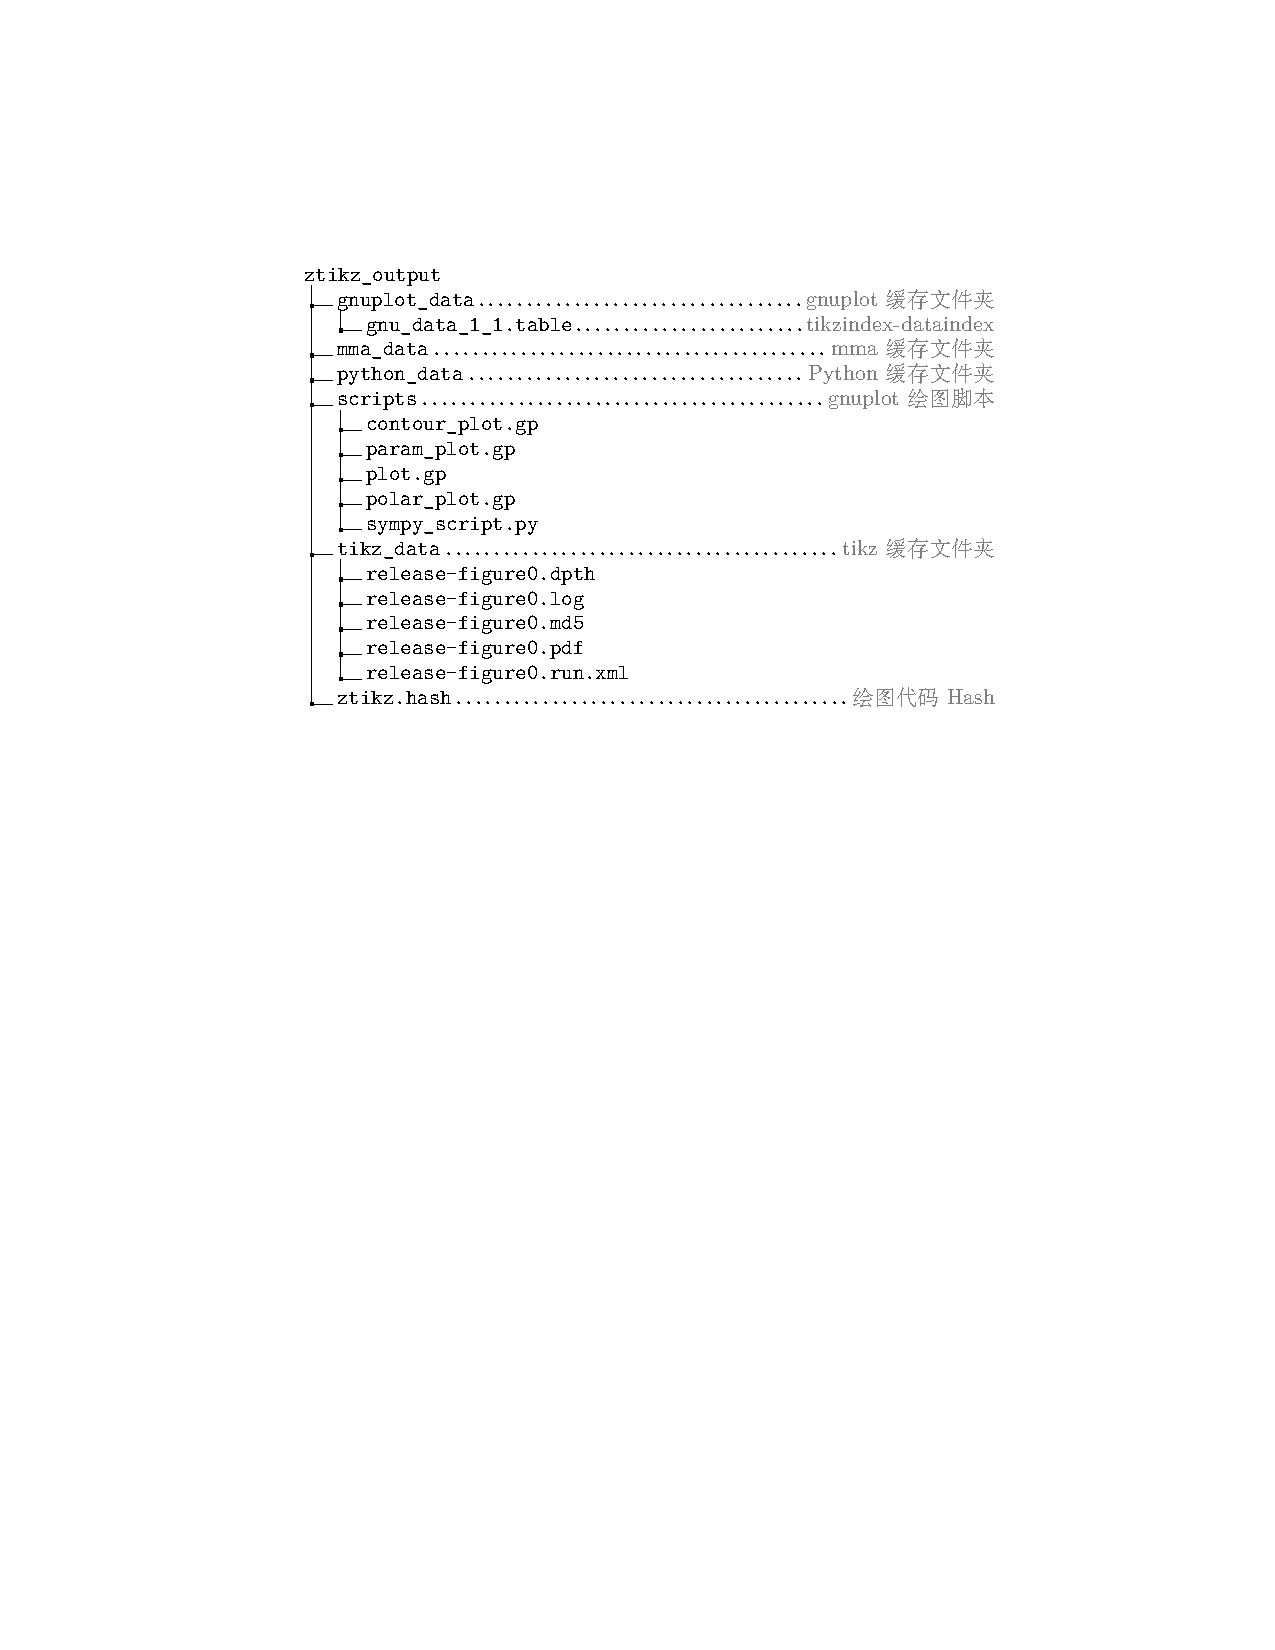
\includegraphics[width=.75\linewidth]{./pics/ztikz_tree.pdf}
    \caption{zTikZ目录结构示意图}
    \label{fig:zTikZ-directory}
\end{figure}

\cmd{tikz_data}中的\cmd{release-figure0.pdf}即为缓存的\cmd{tikzpicture}环境的pdf文件,
对应的\cmd{.md5}文件中:

\begin{codeprint}
\def \tikzexternallastkey {AE7F2539E81C96848ADCCEE3994993D1}%
\end{codeprint}

即保存了\cmd{tikzpicture}环境中代码的Hash Value,当我们改变了\cmd{tikzpicture}环境中的代码时,
这个Hash value就会改变,从而tikz就会再次运行此环境,重新生成图片. 虽说这是tikz自带的功能,但是 
zTikZ中的Cache 机制和这个是十分的类似的,也可以说是一样的. 随便这里在说明一个命令\cmd{\gnudata}
的用法(在后面区域填充时是即为有用的):

\begin{codeprint}
\gnudata{1_2} = ./ztikz_output/gnuplot_data/gnu_data_1_2.table
\end{codeprint}

\cmd{\gnudata}参数中的``1''表示此数据在第一个tikzpicture环境中生成的,``2''表示此数据是在第1个tikzpicture
环境中的第二个绘图数据; 后面我们在解释这个文件夹中其他文件的作用,目前我们先把函数绘制命令\cmd{\Plot}的参数解释清楚。
如果想要设置绘制的函数图形的样式,只需要对其第二个可选项参数进行设置即可,比如设置为``\textcolor{red}{红色}, \textbf{加粗}''.

\begin{codeprint}
\begin{tikzpicture}
    \Plot[-1.5*pi:pi][red, thick]{sin(x)}
\end{tikzpicture}
\end{codeprint}

\begin{center}
    \begin{tikzpicture}
        \Plot[-1.5*pi:pi][red, thick]{sin(x)}
    \end{tikzpicture}
\end{center}


其实上面的第二个参数的值可以是任何合法的\cmd{\draw[<plot style>]}值, 因为每一个函数
绘制命令均是通过如下的命令实现的:

\begin{codeprint}
% gnuplot data rename, plot and precise reset
\cs_new_protected:Npn \ztikz_gnu_data_plot_cs:n #1#2 {
    % rename data file
    \int_gadd:Nn \g__gnu_data_index_int {1}
    \tl_set:Nx \l__gnu_data_new_name_tl {gnu_data_\int_use:N \g__gnu_data_index_int.table}
    \tl_set:Nx \l__gnu_data_full_path_tl {\g__ztikz_gnu_path_tl/\l__gnu_data_new_name_tl}
    \sys_shell_mv:xx {\g__ztikz_gnu_path_tl/gnu_data.table}
                    {\l__gnu_data_full_path_tl}
    % plot data file
    \draw[#2] plot[smooth] file {\l__gnu_data_full_path_tl};
    % reset precise (default 300 for plot precise)
    \bool_if:cTF {g__#1_precise_bool}{
        \PlotPrecise{#1}{300}
    }{\relax}
}
\end{codeprint}

上述函数\cmd{\ztikz_gnu_data_plot_cs:n} 的第二个参数即为\cmd{\Plot}命令的第二个参数;最后在给我们的
图像加上坐标轴等细节: 需要用到绘制坐标轴的\cmd{\ShowAxis}命令, 绘制网格用的\cmd{\ShowGrid}命令,以及
绘制点用的\cmd{\ShowPoint}命令.

其中\index{\cmd{\ShowAxis}}的参数格式为:\cmd{\ShowAxis[<plot style>]{(start coordinate);(end coordinate)}}.
和前面的\cmd{<plot style>}参数相同,任何的\cmd{\draw[<plot style>]}的值都是合法的. \cmd{\ShowAxis}中的第二个参数
表示绘制的坐标轴的起点和终点,使用``\cmd{;}''进行分割(zTikZ 中凡是单个参数中含有多个对象的,分割对象所用到的符号
都是``\cmd{;}''). \index{\cmd{\ShowGrid}}命令的参数也是和\cmd{\ShowAxis}命令的参数一样的,只不过此命令中可以
指定一个\cmd{step}关键字,用于指定绘制网格的步长(间隔), 如\cmd{step=.5},设置步长为0.5. 对应的\index{\cmd{\ShowPoint}}
命令的参数格式为:

\begin{codeprint}
\ShowPoint[<dot style>]{(coordinate 1); (coordinate 2); ...}[<label 1>; <label2>; ...][<position>]
\end{codeprint}

上述的\cmd{<dot style>}通过\cmd{<key>-<value>}的格式进行指定, 可用的\cmd{<key>-<value>}列表为:

\begin{itemize}
    \item \cmd{type}: \cmd{circle, rectangle}, 显示点的形状为圆形/矩形, 默认为circle.
    \item \cmd{radius}: \cmd{<dimension>}, 点的半径,默认为 1pt.
    \item \cmd{color}: \cmd{<color>}, 点的颜色, 默认为black.
    \item \cmd{opacity}: \cmd{<float value>}, 点的透明度,默认为1,即不透明.
\end{itemize}


终于,现在我们可以给出一个相对完整的代码:

\begin{codeprint}
\begin{tikzpicture}[>=Latex]
    \Plot[-1.5*pi:pi][red, thick]{sin(x)}
    \ShowAxis{(-5, 0); (5, 0)}
    \ShowAxis{(0, -2); (0, 2)}
    \ShowGrid[gray, step=1, opacity=.5]{(-5, -2); (5, 2)}
    \ShowPoint[color=orange, radius=1.5pt]{(0, 0); (3.1415926, 0)}[$O=(0, 0)$; $(\pi, 0)$][below right=.5em and .5em]
\end{tikzpicture}
\end{codeprint}

\begin{center}
    \begin{tikzpicture}[>=Latex]
        \Plot[-1.5*pi:pi][red, thick]{sin(x)}
        \ShowAxis{(-5, 0); (5, 0)}
        \ShowAxis{(0, -2); (0, 2)}
        \ShowGrid[gray, step=1, opacity=.5]{(-5, -2); (5, 2)}
        \ShowPoint[color=orange, radius=1.5pt]{(0, 0); (3.1415926, 0)}[$O=(0, 0)$; $(\pi, 0)$][below right=.5em and .5em]
    \end{tikzpicture}
\end{center}

\begin{leftbar}
\noindent \textbf{注意:}zTikZ中的命令都不需要你使用``\cmd{;}''去结束绘制.
\end{leftbar}

其余的几个函数绘制命令,稍微值得一提的是命令\index{\cmd{\ContourPlot}}, 其参数格式为:

\begin{codeprint}
\ContourPlot[<plot domain>][<plot style>]{<function>}
\end{codeprint}

但是因为是 contour plot, 所以它的定义域的指定格式是比较特别的; 比如绘制的定义为:
$-3<x<\pi$ 并且 $-1.5<y<e$. 那么在指定其\cmd{<plot domain>}时应该写为
\cmd{-3:pi;-1.5:exp(1)}.

\begin{leftbar}
\noindent 由于zTikZ的这部分功能都是以gnuplot为基础,所以只要是gnuplot支持的函数,gnuplot内置的任何常数;
你都可以在zTikZ中使用;这里给不熟悉gnuplot的你们推荐一份7页的gnuplot快速
入门清单:\href{http://www.gnuplot.info/docs_4.0/gpcard.pdf}{gnuplot card}
\end{leftbar}

这里就给出一个\cmd{\ContourPlot}的例子,对应的绘图代码见后面:

\begin{center}
    \begin{tikzpicture}[>=Latex, scale=.5]
        \ShowAxis{(-5, 0); (5, 0)}
        \ShowAxis{(0, -5); (0, 5)}
        \ContourPlot[-3:pi; -3:exp(1)][red]{x**2/16 + y**2/10 - 1}
    \end{tikzpicture}
\end{center}

\begin{codeprint}
\begin{tikzpicture}[>=Latex, scale=.5]
    \ShowAxis{(-5, 0); (5, 0)}
    \ShowAxis{(0, -5); (0, 5)}
    \ContourPlot[-3:pi; -3:exp(1)][red]{x**2/16 + y**2/10 - 1}
\end{tikzpicture}
\end{codeprint}

对于\cmd{\ContourPlot}还有一点提醒:如果要绘制 $x^2/4+y^2/9=1$,那么你只需要输入\cmd{x**2/4+y**2/9-1}即可;
所以由此也暗示了此命令的另一个用法,用于绘制水平线($y=c$)和竖直线($x=c$). 仍然可以使用前面的\cmd{<plot domain>}
控制 $x,y$的范围,比如绘制 $x=1, -1<y<1$. 那么对应的命令就是(第一个参数范围只要包含 $x=1$即可):

\begin{codeprint}
\ContourPlot[0:2; -1:1][red, dashed]{x-1}
\end{codeprint}


我们还有两个命令没有讲到:\index{\cmd{\ShowIntersection}}, \index{\cmd{\PlotPrecise}}; 其中\cmd{\ShowIntersection}
命令的参数格式为:

\begin{codeprint}
\ShowIntersection{<path 1>; <path 2>}[<number of points>]
\end{codeprint}

指定tikz中path名称并显示交点方法示例, 我们分别指定两条叫做\cmd{line1, line2}的路径,并显示它们二者的交点.

\begin{codeprint}
\begin{tikzpicture}[>=Latex]
    \ShowAxis{(-2, 0); (4, 0)}
    \ShowAxis{(0, -2); (0, 4)}
    \Plot[1:3][name path=line1]{2*x-3}
    \Plot[0:3][name path=line2]{-x+3}
    \ShowIntersection[color=red]{line1; line2}{1}

    % 可以使用如下的语句
    % \path[name intersections={of=line1 and line2}];
    % \ShowPoint[color=red] {(intersection-1)}
\end{tikzpicture}
\end{codeprint}


\begin{center}
    \begin{tikzpicture}[>=latex]
        \ShowAxis{(-2, 0); (4, 0)}
        \ShowAxis{(0, -2); (0, 4)}
        \Plot[1:3][name path=line1]{2*x-3}
        \Plot[0:3][name path=line2]{-x+3}
        \ShowIntersection[color=red]{line1; line2}{1}
    \end{tikzpicture}
\end{center}


\index{\cmd{\PlotPrecise}}命令的参数格式为:
\begin{codeprint}
\PlotPrecise{<plot type>}[<change domain>]{<samples-int>}
\end{codeprint}

支持的\cmd{<plot type>}有 \cmd{plot, param, contour, polar}, 分别设置对应的
命令\cmd{\Plot, \ParamPlot, \ContourPlot, \PolarPlot}的采样精度. 采样精度的设置
分为两种,临时和永久,临时改变(只改变下一个命令的采样精度)的方法是在命令的第二个参数中
填入\cmd{[once]}, 而如果填入不是\cmd{once},那么接下来的所有同种\cmd{<plot type>}的命令
的采样精度都会改变. 下面给出一个采样精度设置的例子, 绘制在区间$[-2, 2]$上的
函数 $y=3\sin(1/x)$在采样精度分别为50和1000的图像:

\parbox{.48\linewidth}{
    \centering
    \begin{tikzpicture}
        \PlotPrecise{plot}{50}
        \Plot[-2:2]{3*sin(1/x)}
    \end{tikzpicture}
}
\parbox{.48\linewidth}{
    \centering
    \begin{tikzpicture}
        \PlotPrecise{plot}{1000}
        \Plot[-2:2]{3*sin(1/x)}
    \end{tikzpicture}
}

下面我们给出一个运用到zTikZ这部分所有命令的一些综合绘图案例:
\begin{figure}[H]
    \centering
    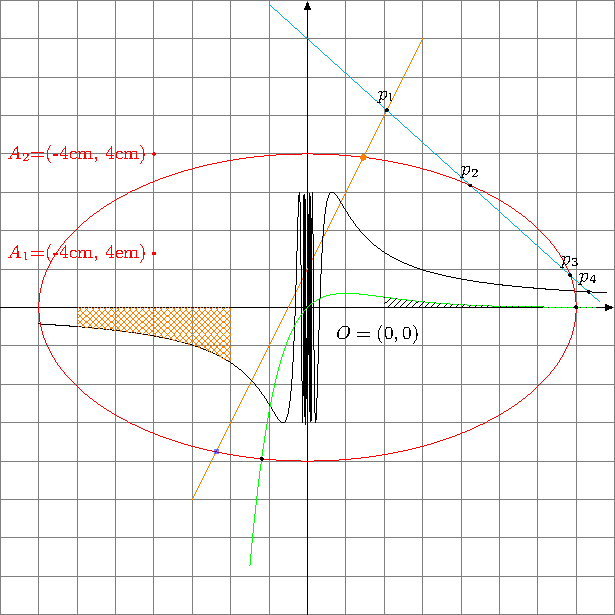
\includegraphics[width=.7\linewidth]{./pics/ztikz_example_1.pdf}
    \caption{绘制示例 1}
    \label{fig:zTikZ-plot—example-1}
\end{figure}


\begin{figure}[H]
    \centering
    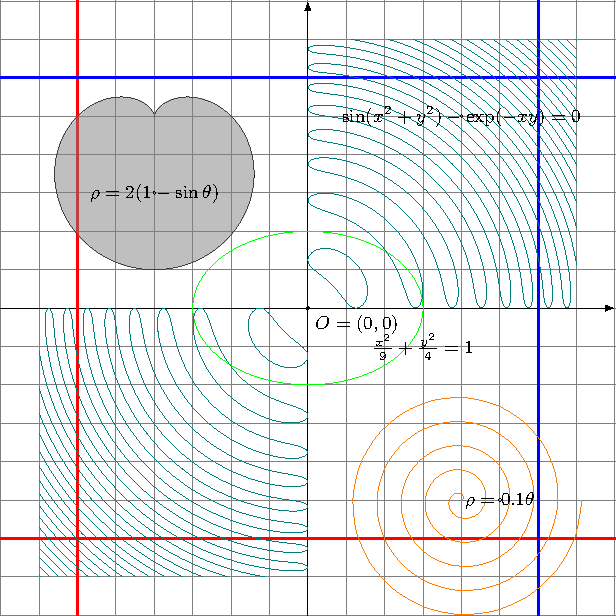
\includegraphics[width=.75\linewidth]{./pics/ztikz_example_2.pdf}
    \caption{绘制示例 2}
    \label{fig:zTikZ-plot—example-2}
\end{figure}


\begin{figure}[H]
    \centering
    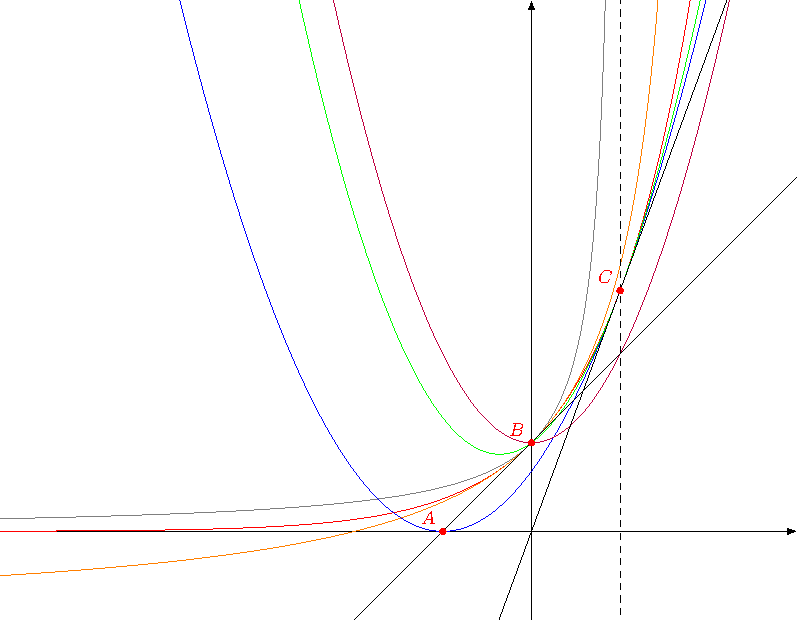
\includegraphics[width=.75\linewidth]{./pics/ztikz_example_3.pdf}
    \caption{绘制示例 3}
    \label{fig:zTikZ-plot—example-3}
\end{figure}

\begin{figure}[H]
    \centering
    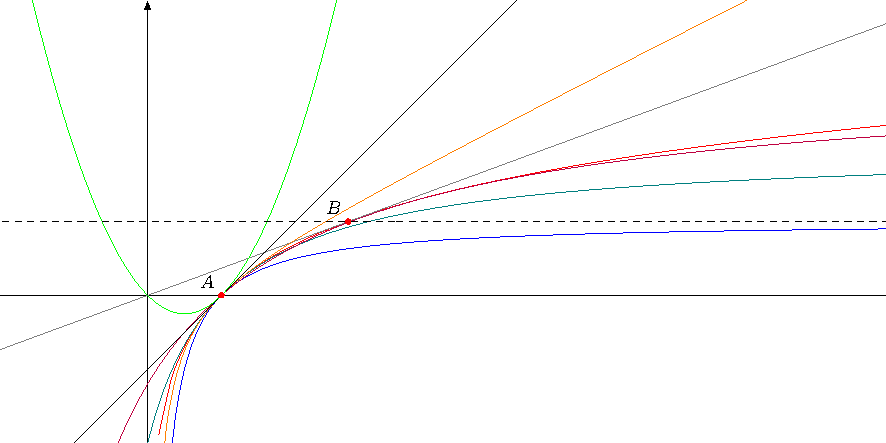
\includegraphics[width=.75\linewidth]{./pics/ztikz_example_4.pdf}
    \caption{绘制示例 4}
    \label{fig:zTikZ-plot—example-4}
\end{figure}

\begin{leftbar}
\noindent 如果你修改了绘图代码,但是发现得到的pdf中的图像并没有改变,那么极有可能是因为
你指定的精度过高,超出了\TeX{}的内存使用限制.(而且由于采用了external库用于缓存,有可能你在编译时都不会抛出
这个错误) 其实比较耗费内存的点主要有3个:
\begin{itemize}
    \item 指定的精度过高, 一般情况下在区间长度$<5$时指定精度为100就已经足够了
    \item 使用了多个\cmd{\ContourPlot}函数,在默认的精度 100下,多个此函数也可能导致内存超出
    \item 最后一点耗时的点就是\cmd{\ShowIntersecion}命令,可以先用Geogebra得到交点后再使用
        \cmd{\ShowPoint}命令进行点的绘制.
\end{itemize}
\end{leftbar}

\subsection{python/matplotlib}
对于python绘图是比较就简单的,zTikZ提供了用于python绘图的\index{\cmd{pyfig}}环境。
此环境需要填入两个参数,参数格式为:

\begin{codeprint}
\begin{pyfig}[<width>]{<export file name>}
% your code
\end{pyfig}
\end{codeprint}

其中的\cmd{<width>}参数是命令\cmd{\includegraphics[<width>]{}}中的参,比如你可以输入\cmd{width=.75\linewidth}. 
再指定必要的参数后,你可以直接在环境中输入Python代码. 下面即为一个示例:

\begin{codeprint}
\begin{pyfig}[width=.45\linewidth]{pycode.py}
import matplotlib 
matplotlib.use('Agg')
from matplotlib import pyplot as plt
plt.rcParams['font.sans-serif'] = ['FangSong']  
plt.rcParams['axes.unicode_minus'] = False
import numpy as np

x = np.linspace(0, 2*np.pi, num = 80)
y = np.sin(x)*np.cos(x)+.2
plt.plot(x, y)
\end{pyfig}
\end{codeprint}

你不需要在其中输入图片的保存指令\cmd{plt.savefig("")}, zTikZ会自动在此环境后面加上对应的
图片保存指令。这个环境的返回结果为:\cmd{\includegraphics[width=.45\linewidth]{pycode.py.pdf}},
所以你可以把这个环境嵌套在任何的浮动环境,比如\cmd{figure, table}中. 

在命令行中第一次编译时你会看到如下的日志:
\begin{codeprint}
current hash is FF7B5ECDBF52AA95DF921FCC076F9021
current hash is unique --> recorded
\end{codeprint}

上述日志说明,zTikZ已经识别到这是一个新的python环境,并且保存了这个环境中绘图代码的Hash值;
然后,第二次编译此文档时,你会在输出的日志中定位到如下的输出:
\begin{codeprint}
current hash is FF7B5ECDBF52AA95DF921FCC076F9021
skip recompile by python, using the cache picture 1
\end{codeprint}

这就说明,由于你的python绘图部分的源代码没有改变,然后zTikZ就直接采用了上一次编译的缓存图片,跳过了重新编译这一步;
上面环境的运行结果为:

\begin{figure}[!htb]
    \centering
\begin{pyfig}[width=.75\linewidth]{pycode.py}
import matplotlib 
matplotlib.use('Agg')
from matplotlib import pyplot as plt
plt.rcParams['font.sans-serif'] = ['FangSong']  
plt.rcParams['axes.unicode_minus'] = False
import numpy as np

x = np.linspace(0, 2*np.pi, num = 80)
y = np.sin(x)*np.cos(x)+.2
plt.plot(x, y)
\end{pyfig}
    \caption{Python绘图示例 1}
    \label{fig:py-fig-1}
\end{figure}

这里再给一个Python绘图环境的示例,绘制了一个简单的来自Matplotlib官方的三位图像. 
其实这里给出这个例子,就是为了让读者明白,尽管目前zTikZ还没有支持便捷的三维矢量图形绘制,
但是你可以使用Python生成对应的3维矢量图;虽然,你可能需要再去学习Python中Matplotlib的
相关语法,但是这是简单的.

\begin{figure}[!htb]
    \centering
    \input{./data/pyfig_II.mpl}
    \caption{Python绘图示例 2}
    \label{fig:py-fig-2}
\end{figure}

\begin{leftbar}
由于python是依靠缩进来识别代码结构的,所以在书写这部分的代码时,不能够人工添加缩进,在书写的时候
需写为下面这样:
\begin{center}
    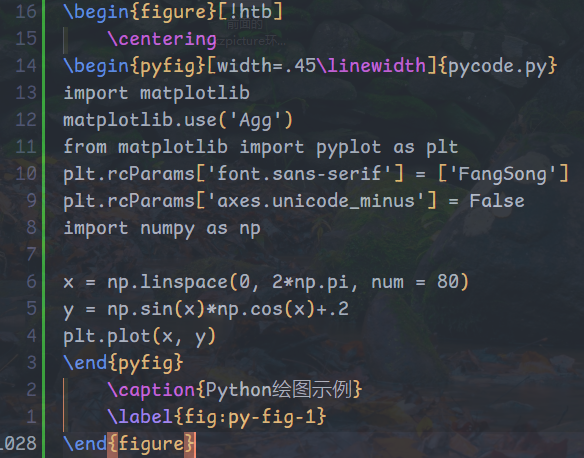
\includegraphics[width=.45\linewidth]{./pics/pyfig_example.png}
\end{center}

如果你实在是需要缩进,那么在这里我推荐另外一种一种可以使用缩进的方法;把\cmd{pyfig}环境连同其内部代码保存在另外一个文件中,
比如这里我保存为\cmd{pycode.mpl},然后在\cmd{figure}环境中使用\cmd{\input{pycode.mpl}}引入此部分的代码。如下:
\begin{codeprint}
\begin{figure}
    \centering
    \input{./data/pycode.mpl}
    \caption{Python Figure}
    \label{fig:pyfig-1}
\end{figure}
\end{codeprint}
\end{leftbar}


\subsection{mathematica}
其实使用mathematica进行绘图这个部分和前面的使用Python绘图是差不多的,zTikZ提供了一个
\index{\cmd{mmafig}}环境用于使用mathematica绘图. 与之前的\cmd{pyfig}环境不同的是,此时你需要手动加入
图片的保存路径;路径的前缀为:\cmd{./ztikz_output/mma_data/<figure name>}. 为何这里这个部分
我不使用zTikZ自动完成? 由于mathematica绘图代码中可能存在着多辐图形的情况,需要使用\cmd{Show}命令
组合成为一个图,那么这个组合方式就是千变万化的了。所以为了给用户提供给更多的自由操作的空间。
这里的图片保存命令由用户自己书写. 并且上述的\cmd{<figure name>}只能写为\cmd{<wls script name>.pdf}
的形式;比如你的WolframScript脚本名称为\cmd{mma_1.wls},那么你的\cmd{<figure name>}只能写为
\cmd{mma_1.wls.pdf},其中的图片格式可以自己指定,比如为\cmd{.png, .jpg, .mbp}等. 此环境同样是加入了Cache机制的,
下面给出一个具体的使用案例:

\begin{codeprint}
\begin{mmafig}[width=.4\linewidth]{mma_1.wls}
    plotFunction[fun_, xlimits_, ylimits_] := ContourPlot[fun, 
        xlimits, ylimits,
        ContourStyle->{
            RGBColor["#00C0A3"], 
            Thickness[0.004]
        },
        AspectRatio->((xlimits[[2]]//Abs) + (xlimits[[3]]//Abs))/((ylimits[[2]]//Abs) + (ylimits[[3]]//Abs)), 
        AxesOrigin->{0,0}, 
        Axes->True,
        Frame->False,
        AxesStyle->Arrowheads[{0, 0.03}],
        AxesLabel->{"x", "y"},
        PlotRange -> Full
    ]
    
    xlimits = {x, -3, 6};
    ylimits = {y, -4, 5};
    fp1 = plotFunction[y==Sin[x], xlimits, ylimits];
    fp2 = plotFunction[x^2/4 + y^2/3 == 5, {x, -5, 5}, {y, -5, 5}];
    
    figure = Show[fp2, fp1];
    (* 1.保存的图片格式为:*.wls.pdf; 2.保存路径在:./ztikz_output/mma_data *)
    Export["./ztikz_output/mma_data/mma_1.wls.pdf", figure];
\end{mmafig}
\end{codeprint}

因为mathematica中的代码是允许用户自由添加缩进的,所以你可以自己添加Mathematica代码的缩进.
和前面的Python绘图代码类似,你可以把此部分代码保存在一个单独的文件中,然后通过\cmd{\input}
进行引入,这里不再给出对应的案例.

\begin{leftbar}
\textbullet 注意空格与Tab,如果源代码中有Tab,那么zTikZ在进行此环境的抄录时会把原本
的Tab转义为 \verb|^^I|,从而造成Mathematica源代码的错误, 比如你可能会看到你的源代码
抄录后变成了下面的样子:
\begin{verbatim}
^^IContourStyle->{
^^I^^IRGBColor["#00C0A3"], 
^^I},
\end{verbatim}

\textbullet 同时注意Mathematica中注释的写法, 不是\verb|(* something*)|, 而是\verb|(* something *)|,
也就是你的注释不能够紧挨着 \verb|*|, 否则会造成mathematica script的解析错误.

\textbullet 由于WolframScript的限制,对应的Mathematica脚本的后缀只能为:\cmd{.wls},否则WolframScript
无法识别此脚本,也就不会去执行此脚本了.
\end{leftbar}


\begin{figure}[!htb]
    \centering
    \begin{mmafig}[width=.5\linewidth]{mma_1.wls}
        plotFunction[fun_, xlimits_, ylimits_] := ContourPlot[fun, 
            xlimits, ylimits,
            ContourStyle->{
                RGBColor["#00C0A3"], 
                Thickness[0.004]
            },
            AspectRatio->((xlimits[[2]]//Abs) + (xlimits[[3]]//Abs))/((ylimits[[2]]//Abs) + (ylimits[[3]]//Abs)), 
            AxesOrigin->{0,0}, 
            Axes->True,
            Frame->False,
            AxesStyle->Arrowheads[{0, 0.03}],
            AxesLabel->{"x", "y"},
            PlotRange -> Full
        ]
        
        xlimits = {x, -3, 6};
        ylimits = {y, -4, 5};
        fp1 = plotFunction[y==Sin[x], xlimits, ylimits];
        fp2 = plotFunction[x^2/4 + y^2/3 == 5, {x, -5, 5}, {y, -5, 5}];
        
        figure = Show[fp2, fp1];
        (* 1.保存的图片格式为:*.wls.pdf; 2.保存路径在:./ztikz_output/mma_data *)
        Export["./ztikz_output/mma_data/mma_1.wls.pdf", figure];
    \end{mmafig}
    \caption{Mathematica 绘图示例}
    \label{fig:mma-fig-1}
\end{figure}

同样的你可以使用Mathematica绘制3维图形\Footnote{由于目前的Mathematica不支持输出3维矢量图,所以想要 
是你的3维图像显得更加的清晰,可以调节图像的分辨率.}。目前zTikZ仅支持插入静态图片,后续可能会考虑加入 
动态图片的支持功能,就行另外一个开源矢量图象绘制软件\href{https://asymptote.sourceforge.io/}{Asymptote}
中的\cmd{.prc}文件一样. 但是要是的PDF支持动态图形,首先你的PDF阅读器必须支持JavaScript,常见的
这种类型的PDF阅读器就是Adobe家的Acrobat了.

\begin{figure}[!htb]
    \centering
    \input{./data/mma_2.wls}
    \caption{Mathematica绘图示例 2}
    \label{fig:mma-fig-2}
\end{figure}


\section{数值计算}
\subsection{xfp}
众说周知,\TeX{}自身的计算能力是比较若的,所以涉及到一定的计算需求时,一般宏包的解决方法都是
使用外部程序,让\TeX{}只负责排版就行了.但是在\LaTeX3项目发展了这么久之后,也做出了一些令人 
惊喜的结果。这里我们主要介绍\LaTeX3的 \href{https://www.ctan.org/pkg/xfp}{xfp} 宏包,用于浮点数运算. 

这里说明部分\index{\cmd{xfp}}也许可以解决的痛点: 
\begin{itemize}
    \item 在TikZ绘图中,常常时需要坐标运算的,尽管TikZ提供了一个\cmd{calc}库,但是
        这个库的使用语法总觉得不是那么的自然。于是这个时候你就可以使用\cmd{xfp}宏包.
    \item 在你自定义一些需要用到数值计算的宏命令时,使用\cmd{xfp}宏包是一个比较好的选择.
\end{itemize}

\cmd{xfp}宏包的详细使用教程请参见官方文档,这里不再赘述.

\begin{leftbar}
\noindent zTikZ或者是z\LaTeX{}并不会自动加载\cmd{xfp}宏包,如果你有这方面的需要,请自己加载.
\end{leftbar}

\subsection{python}
上面介绍了Python的绘图功能,这里再引入zTikZ中的浮点数计算部分(Sympy对应的部分应该不能叫浮点数计算了,毕竟Sympy
进行的是精确的计算。)这里使用的浮点数运算主要是基于Python,以及可能的宏包\cmd{numpy}等. zTikZ在调用
此命令是默认载入Python库\cmd{NumPy, SciPy},并且使用\cmd{numpy}中的函数时不用再加上前缀;比如求解$\sin(2.345)$
时,直接使用\cmd{\pyfp{sin(2.345)}}即可,不用写成\cmd{\pyfp{np.sin(2.345)}}.对于库\cmd{SciPy}中的函数
使用方法同理.

zTikZ提供了命令\index{\cmd{\pyfp}}用于浮点数运算, 这部分的结果并不会被缓存,也就是说每次编译此文档时,Python都会重新
计算此部分的结果. \cmd{\pyfp}的参数说明如下:

\begin{codeprint}
\pyfig{<expression>}
\end{codeprint}

下面给出一个使用样例:
\begin{codeprint}
\pyfp{0.9**10}
\end{codeprint}

\[
    0.9^{10} = \pyfp{0.9**10}
\]


\subsection{mathematica}
使用Mathematica进行数值计算这一部分和后面的\index{\cmd{\wolfram}}指令是有一部分重合的,详细的使用参见后面一节的
``符号计算'', 所以这一部分我们就在后面介绍.


\section{符号计算}
符号计算是区别于数值计算的,上述的数值计算章节应该也有介绍; 但在介绍zTikZ中的符号计算模块之前先给出一个
符号计算的定义,以下定义摘自wiki:

\begin{leftbar}
\kaishu 数学和计算机科学中,计算机代数或符号计算或代数计算,是研究、开发用于操作表达式等数学对象的算法与软件的科学领域。
这通常被视为是运算科学的一个子领域,但运算科学一般基于近似浮点数的数值计算,而符号计算则使用含变量的表达式进行精确计算,
其中变量没有赋值。 执行符号计算的软件系统称为计算机代数系统(computer algebra system, CAS),``系统''暗示了软件的复杂性,
其中至少包括一种在计算机中表示数学数据的方法、一种编程语言(通常异于用于实现的语言)、一种专门的内存管理器、
一套供输入输出表达式的用户界面、一大套用于通常运算的子程序,如表达式简化、能实现链式法则、多项式因式分解、
不定积分等等的求导算法。
\end{leftbar}

当前流行的计算机代数系统主要有:
\begin{multicols}{2}
    \begin{itemize}
    \item mathHandbook.com
    \item Sagemath
    \item Mathematica
    \item Maple
    \item MAGMA
    \item Maxima
    \item GAP
    \item PARI/GP
    \item Meditor
    \item MuPAD
    \item Mathomatic
    \item Xcas/Giac
    \item Yacas
    \item Mate
    \end{itemize}
\end{multicols}

zTikZ主要提供一个和Mathematica(假如你已经购买了该软件),以及Pyhton的Sympy模块的符号计算接口.
后续可能会开发一个统一的接口用于\TeX{}和外部程序的交互.

\subsection{python/sympy}
Python的Sympy是一个\textbf{免费,开源,轻量}的符号计算模块,其官网上有着详细的\href{https://docs.sympy.org/latest/tutorials/intro-tutorial/index.html}{教程}。
所以这里便不再赘述其语法,重点介绍zTikZ中提供的几个接口(命令),用于和Sympy交互.

zTikZ中针对Sympy提供了命令:\index{\cmd{\sympy}},其参数格式为:

\begin{codeprint}
\sympy{<expression>}
\end{codeprint}

和之前的使用Python进行数值计算不同的是,zTikZ针对此命令提供了Cache机制,此命令对应的结果会被保存在文件:
\cmd{./ztikz_output/python_data/sympy_<index>.out}文件中. 此文件名中的\cmd{<index>}表示的是对应的
符号计算表达式的序号. 

\cmd{\sympy}命令的运算结果被保存在文件中之后,通过\cmd{\input}命令把对应的运算结果导入到\TeX{}的输出流(文档)中,
由于默认的情况下此结果包含数学公式中的上下标:\cmd{^, _, ...}等, 所以在把其导入到\LaTeX{}源码中时需要放入数学环境中.

zTikZ模块的\cmd{\sympy}命令在进行符号运算时,默认的符号变量有:\cmd{x, y, z, u, v, t},这些变量你不需声明
便可以直接使用; 下面给出使用\cmd{\sympy}命令进行符号计算的部分示例:

\begin{codeprint}
% 定积分
\sympy{integrate(sin(x)/x, (x, -oo, oo))}
% 不定积分
\sympy{integrate( x**8 + cos(7*x) + 6*t, x )}
% 矩阵特征值
\sympy{Matrix([[1, 2], [2, 2]]).eigenvals()}  
% 极限计算
\sympy{limit(sin(x)/x, x, 0)}
\end{codeprint}

计算定积分的例子:
\[
\int_{-\infty}^{+\infty}{\frac{\sin(x)}{x} \;\mathrm{d}x}
    = \sympy{integrate(sin(x)/x, (x, -oo, oo))}      
\]   

或者是计算不定积分的例子:
\[
    \int x^8 + \cos(7x) + 6t\,\mathrm{d}x  
    = \sympy{integrate( x**8 + cos(7*x) + 6*t, x )}    
\]

或者是一个计算特征值的例子:
\[
\mathrm{eig}(\begin{bmatrix}1 & 2\\2 & 2\end{bmatrix})
    = \sympy{Matrix([[1, 2], [2, 2]]).eigenvals()}    
\]

计算极限的例子:
\[
\lim_{x\to 0}{\frac{\sin x}{x}}
    = \sympy{limit(sin(x)/x, x, 0)}    
\]

\begin{leftbar}
\noindent 目前的\cmd{\sympy}命令只支持单行命令的模式,如果你需要使用多行(条)命令来达到计算目的,
请考虑把它们变为一行命令(一条指令).
\end{leftbar}


\subsection{mathematica}
zTikZ模块提供和Mathematica相关的符号计算,数值运算和知识查询接口; 以下的所有命令均具有缓存机制.
\begin{itemize}
    \item \cmd{\wolfram[<option>]{<expression>}}: 使用Mathematica计算此表达式\cmd{<expression>},默认返回
        \TeX{}格式的代码,可以把\cmd{<option>}设为\cmd{text},让其返回一个文本对象. 可以在这个命令中执行
        任何的wolfram指令,但是需要注意的一点是,所有和wolfram相关的命令是不会自动进入数学模式的,需要手动
        添加数学模式的标记.
    \item \cmd{\wolframsolve[<cmd style>]{<expression>}[<varible>][<domain>]}:其中第一个可选参数默认值为:
        \cmd{part},意味着你的命令需要分拆为3个部分:表达式 -- (求解)变量名 -- 求解范围,对应上面的参数,分别填入。
        如果指定第一个参数为\cmd{full},那么此时只需要给出对应的\cmd{<expresion>},不用在指定后续的参数.(毕竟在
        第二个(强制性-Mandatory)参数中就已经包含了这些信息,参见后面的具体使用样例).
    \item \cmd{\wolframdsolve[<cmd style>]{<equation>}[<independent varible>][<dependent variablei>]}:
        此命令用于求解微分方程,其中的第一个可选参数和上面的\cmd{\wolframsolve}的意义一致,不再赘述.第二个参数表示
        要求解的微分方程,第三个参数表示求解的独立变量(函数),最后一个参数表示此微分方程求解函数的自变量.
\end{itemize}

\subsubsection{wolfram}
首先给出\index{\cmd{\wolfram}}命令的部分使用样例:

\begin{codeprint}
\wolfram{Series[Exp[x], {x, 0, 5}]}
\wolfram{LaplaceTransform[t^4 Sin[t],t,s]}  
\wolfram[text]{WolframAlpha["Shanghai population", "ShortAnswer"]} 
\end{codeprint}

函数 $y=\mathrm{e}^x$的5阶Taylor展开式为:
\[
    \wolfram{Series[Exp[x], {x, 0, 5}]}    
\]

函数 $x=t^4 \sin(t)$的Laplace变换为:
\[
    \C{L}[t^4 \sin(t)] = \wolfram{LaplaceTransform[t^4 Sin[t],t,s]}    
\]

在\cmd{\wolfram}指令中执行Mathematica中的\cmd{WolframAlpha}命令进行查询,比如这里查询
上海的人口数量,结果为:\wolfram[text]{WolframAlpha["Shanghai population", "ShortAnswer"]}

这里补充一个使用\cmd{\wolfram}就行数值运算的例子,因为Mathematica 中有着诸多的和数值运算的函数,
这里仅以内置的函数\cmd{N[<expression>]}为例: 

比如我们求解 $\pi$的截取前30小数的近似值为:
\[
    \pi \approx \wolfram{N[Pi, 30]}    
\]

\begin{leftbar}
\noindent 在使用\cmd{\wolfram}命令进行浮点数运算时,只要表达式中含有小数,那么Mathematica就会默认进行浮点数
运算,而不会计算表达式的精确值.
\end{leftbar}

\subsubsection{wolframsolve}
\index{\cmd{\wolframsolve}}命令可以用于多项式方程根的求解以及方程组的求解,并且可以给定求解的范围.
和前面的\cmd{\wolfram}命令类似,此命令\textbf{只}返回求解结果的\TeX{}代码,所以请把此命令置于公式环境中; 
下面给出几个比较简单的求解示例:

\begin{codeprint}
\wolframsolve{x^4 - x^2 - 5 == 0}{x}
\wolframsolve{a x + y == 7 && b x - y == 1}{x, y}
\wolframsolve{x^2 + 2 y^3 == 3681 && x > 0 && y > 0}[x, y][Integers] 
\wolframsolve[full]{x^2 + y^2 == 5^2 && y > x > 0, {x, y}, Integers}  
\end{codeprint}
    
方程 $x^4 - x^2 - 5 == 0$的所有根为:
\[
    \wolframsolve{x^4 - x^2 - 5 == 0}[x]
\]

方程组 $\left\{\begin{aligned}& a x + y == 7\\ & b x - y == 1\end{aligned}\right.$ 的解为:
\[
    \wolframsolve{a x + y == 7 && b x - y == 1}[x, y]
\]

不定方程 $\left\{\begin{aligned}& x^2 + 2 y^3 == 3681 \\ & x > 0, y>0\end{aligned}\right.$ 的整数解为:
\[
    \wolframsolve{x^2 + 2 y^3 == 3681 && x > 0 && y > 0}[x, y][Integers]    
\]

不定方程 $\left\{\begin{aligned}& x^2 + y^2 == 5^2 \\ & x > y > 0\end{aligned}\right.$ 的整数解为:
\[
    \wolframsolve[full]{x^2 + y^2 == 5^2 && y > x > 0, {x, y}, Integers}    
\]

\begin{leftbar}
\noindent 后续可能会考虑加入解的筛选等功能,其实就是根据不同解之间的分隔符 `,'来对返回的字符串进行一个划分.
根据划分的结果生成一个列表,然后采用一个整数进行索引.
\end{leftbar}

\subsubsection{wolframdsolve}
命令\index{\cmd{\wolframdsolve}}和命令\cmd{\wolframsolve}完全相同, 只是这个命令是用于求解微分方程的.
下面是几个示例:

\begin{codeprint}
\wolframdsolve{{y'[x] + y[x] == a*Sin[x], y[0] == 0}}[y[x]][x]   
\wolframdsolve[full]{{y'[x]==Exp[z[x]]+1, z'[x]==y[x]-x}, {y,z}, x}
\end{codeprint}

微分方程 $y' + y = a\sin(x), y(0)=0$的解为:
\[
    \wolframdsolve{{y'[x] + y[x] == a*Sin[x], y[0] == 0}}[y[x]][x]     
\]

非线性系统微分方程组$y'(x) + y(x) = \mathrm{Exp}(z(x))+1, z'(x) = y(x)-x$的解为:
\[
    \wolframdsolve[full]{{y'[x] == Exp[z[x]] + 1, z'[x] == y[x] - x}, {y[x], z[x]}, x}
\]



\chapter{致谢}
\section{(L\raise2.5pt\hbox{a})\TeX{}}
Wiki上对\TeX{}的定义:
\begin{leftbar}
    TeX (\texttt{/t$\varepsilon$x/}), stylized within the system as \TeX{}, is a typesetting system which was designed 
    and written by computer scientist and Stanford University professor \href{https://en.wikipedia.org/wiki/Donald_Knuth}{Donald Knuth} 
    and first released in 1978. \TeX{} is a popular means of typesetting complex mathematical formulae; 
    it has been noted as one of the most sophisticated digital typographical systems.
\end{leftbar}

但是在我看来\TeX{}不仅仅只是一个排版系统,他是一种精神,一种对于美的追求,一种对于细节的关注.
他并不是\cmd{$Word$}那种商业工具,更不是随性MarkDown.(这里不去谈论\textbf{方正}) 在\TeX{}的基础上
建立了一种格式\LaTeX{}, 这种格式更加的人性化,更加的易用. 使得我们普通人也可以使用部分\TeX{}的排版功能.
为何还有人说\LaTeX{}难学呢 ? 假如他用过\TeX{}之后就会明白\LaTeX{} 的平易近人了.


\section{(L\raise2.5pt\hbox{a})\TeX{}社区}
在此还要感谢所有的 \TeX{} 社区,正是因为他们的无私奉献,本系列才能够顺利的完成. 更特别
感谢 \href{https://www.latex-project.org/latex3/}{\LaTeX3} 团队的所有成员.



\addcontentsline{toc}{chapter}{部分名词索引}
\printindex

\end{document}"' ========

! Package tikz Error: Sorry, the system call 'pdflatex -halt-on-error -interact
ion=batchmode -jobname "tikzdata/release-figure0" "\def\tikzexternalrealjob{release}\i
nput{release}"' did NOT result in a usable output file 'tikzdatamain-figure0' (exp
ected one of .pdf:.jpg:.jpeg:.png:). Please verify that you have enabled system
    calls. For pdflatex, this is 'pdflatex -shell-escape'. Sometimes it is also na
med 'write 18' or something like that. Or maybe the command simply failed? Erro
r messages can be found in 'tikzdata/release-figure0.log'. If you continue now, I'l
l try to typeset the picture.
\end{codeprint}

关于此问题我已经在Github上给作者提了\href{https://github.com/maieul/indextools/issues/17}{Issue},
同时也在\TeX-SE上发出了\href{https://tex.stackexchange.com/questions/712716/indextools-confilict-with-tikz-library-external}{提问}.
可以关注上述的问题找到解决方法.

目前的解决方法有两个:
\begin{itemize}
    \item 取消加载indextools宏包,改用传统的\cmd{makeidx}宏包.(需自行去修改\cmd{zlatex.cls}中的加载项)
    \item 仍然使用此宏包,但是在第一遍(tikz图片还没有缓存时)取消导言区以及文档末尾的如下命令:
\begin{codeprint}
% 导言区
\makeindex[title=Test Title, columns=3]
% 文末
\addcontentsline{toc}{chapter}{部分名词索引}
\printindex
\end{codeprint}
        然后在文档的第二次编译时取消两处命令的注释,以此达到正常编译的目的.
\end{itemize}

\begin{leftbar}
\noindent 为何我一再坚持使用\cmd{indextools}宏包? 相较于传统的\cmd{makaidx}宏包需要在命令行中
先使用\LaTeX{}引擎编译,然后使用\cmd{makeindex}命令编译,最后再使用\LaTeX{}引擎编译两遍。\cmd{indextools}
宏包可以在不超过两次的\LaTeX{}引擎编译下直接生成对应的index,方便了许多.
\end{leftbar}